\documentclass{beamer}
\usepackage[latin1]{inputenc}
\usepackage{amsfonts}
\usepackage{listings}
\usepackage{hyperref}
\usepackage{graphicx}
%\usetheme{Luebeck}
\usetheme{Warsaw}
\title[Kinect Controlled Robotic Arm]{Kinect Controlled Robotic Arm}
\author{Aayush Singhal  (aayush@cse)    09005041 \\ \and
        Sivakanth Gopi  (gopisivakanth@cse) 09005043 \\ \and
        Sriram Bhargav Karnati  (ram@cse)   09005067 \\\and
        Aakash Rao N S  (aakash@cse)    09005069}
\date{}
\begin{document}
\begin{frame}
\titlepage
\begin{center}
Group 10\\
CS308 $-$ Embedded Systems Lab\\
IIT Bombay
\end{center}
\end{frame}

\section{Project Idea}
\begin{frame}{Motivation}
\begin{itemize}
\item[-] Controlling a robotic arm with a traditional controller can be very difficult
\item[-] Non-intuitive and increases the complexity of operation
\end{itemize}
What we need is a Natural User Interface (NUI)
\begin{itemize}
\item[-] With NUI the human arm can directly control the robotic arm which tries to imitate its movements
\item[-] Thus controlling the arm becomes very intuitive 
\item[-] User should able to deploy the arm in remote or hostile places
\item[-] Opens a plethora of applications
\end{itemize}
\end{frame}
\begin{frame}{Kinect}
  \begin{figure}
      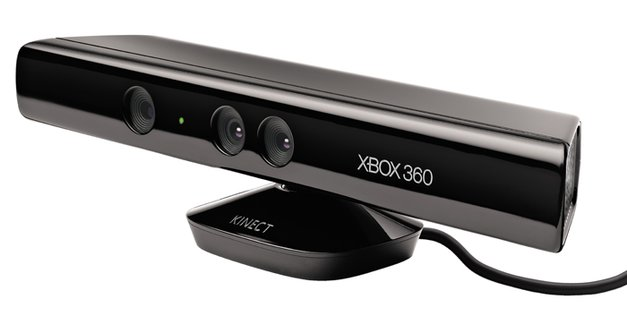
\includegraphics[scale = .4]{kinect.jpg}
      \caption{Microsoft Kinect} 
  \end{figure}

\end{frame}

\begin{frame}{Project Idea}
Provide a NUI for remotely controlling  a robotic arm
\begin{itemize}
\item[-]live video feed from a camera placed on the robotic arm is transmitted by wireless to computer
\item[-]user responds by moving his arms and making gestures
\item[-]movements and gestures of human arm are captured using kinect
\item[-]converted into controls for robotic arm which are transmitted to the arm
\item[-]robotic arm imitates the human arm
\end{itemize}
\end{frame}

\section{Robotic Arm}
\begin{frame}
  \begin{table}
  \begin{tabular}{|l|l|l|}
      \hline
      Axis & Function\\
      \hline
      1 & Base Rotation\\
      2 & Shoulder Rotation\\
      3 & Elbow Rotation\\
      4 & Wrist Pitch\\
      5 & Wrist Roll\\
      6 & Grip,Ungrip\\
      \hline
    \end{tabular}
    \end{table}
  \begin{figure}
      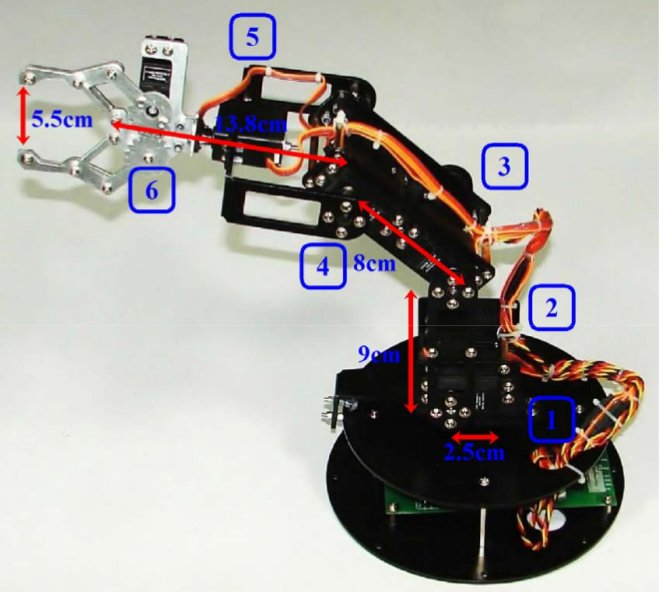
\includegraphics[scale = .2]{arm-axes.jpg}
      %\caption{Dexter ER2 Robotic Arm} 
  \end{figure}      
  
  
\end{frame}
\section{Key Challenges}
\begin{frame}{Challenges}
\begin{itemize}
\item Design an intuitive and robust NUI for arm control. Problems:
\begin{itemize}
\item[-]kinect cannot capture finger movements and wrist roll
\item[-]human shoulder has two axis of rotation
\item[-]kinect skeletal data may not be very accurate
\end{itemize}
\item Establish wireless communication with robotic arm
\item Transmit live video feed from robotic arm
\end{itemize}
\end{frame}
\section{Response}
\subsection{Gestures}
\begin{frame}{Zero Position}
  \begin{figure}
      \centering
      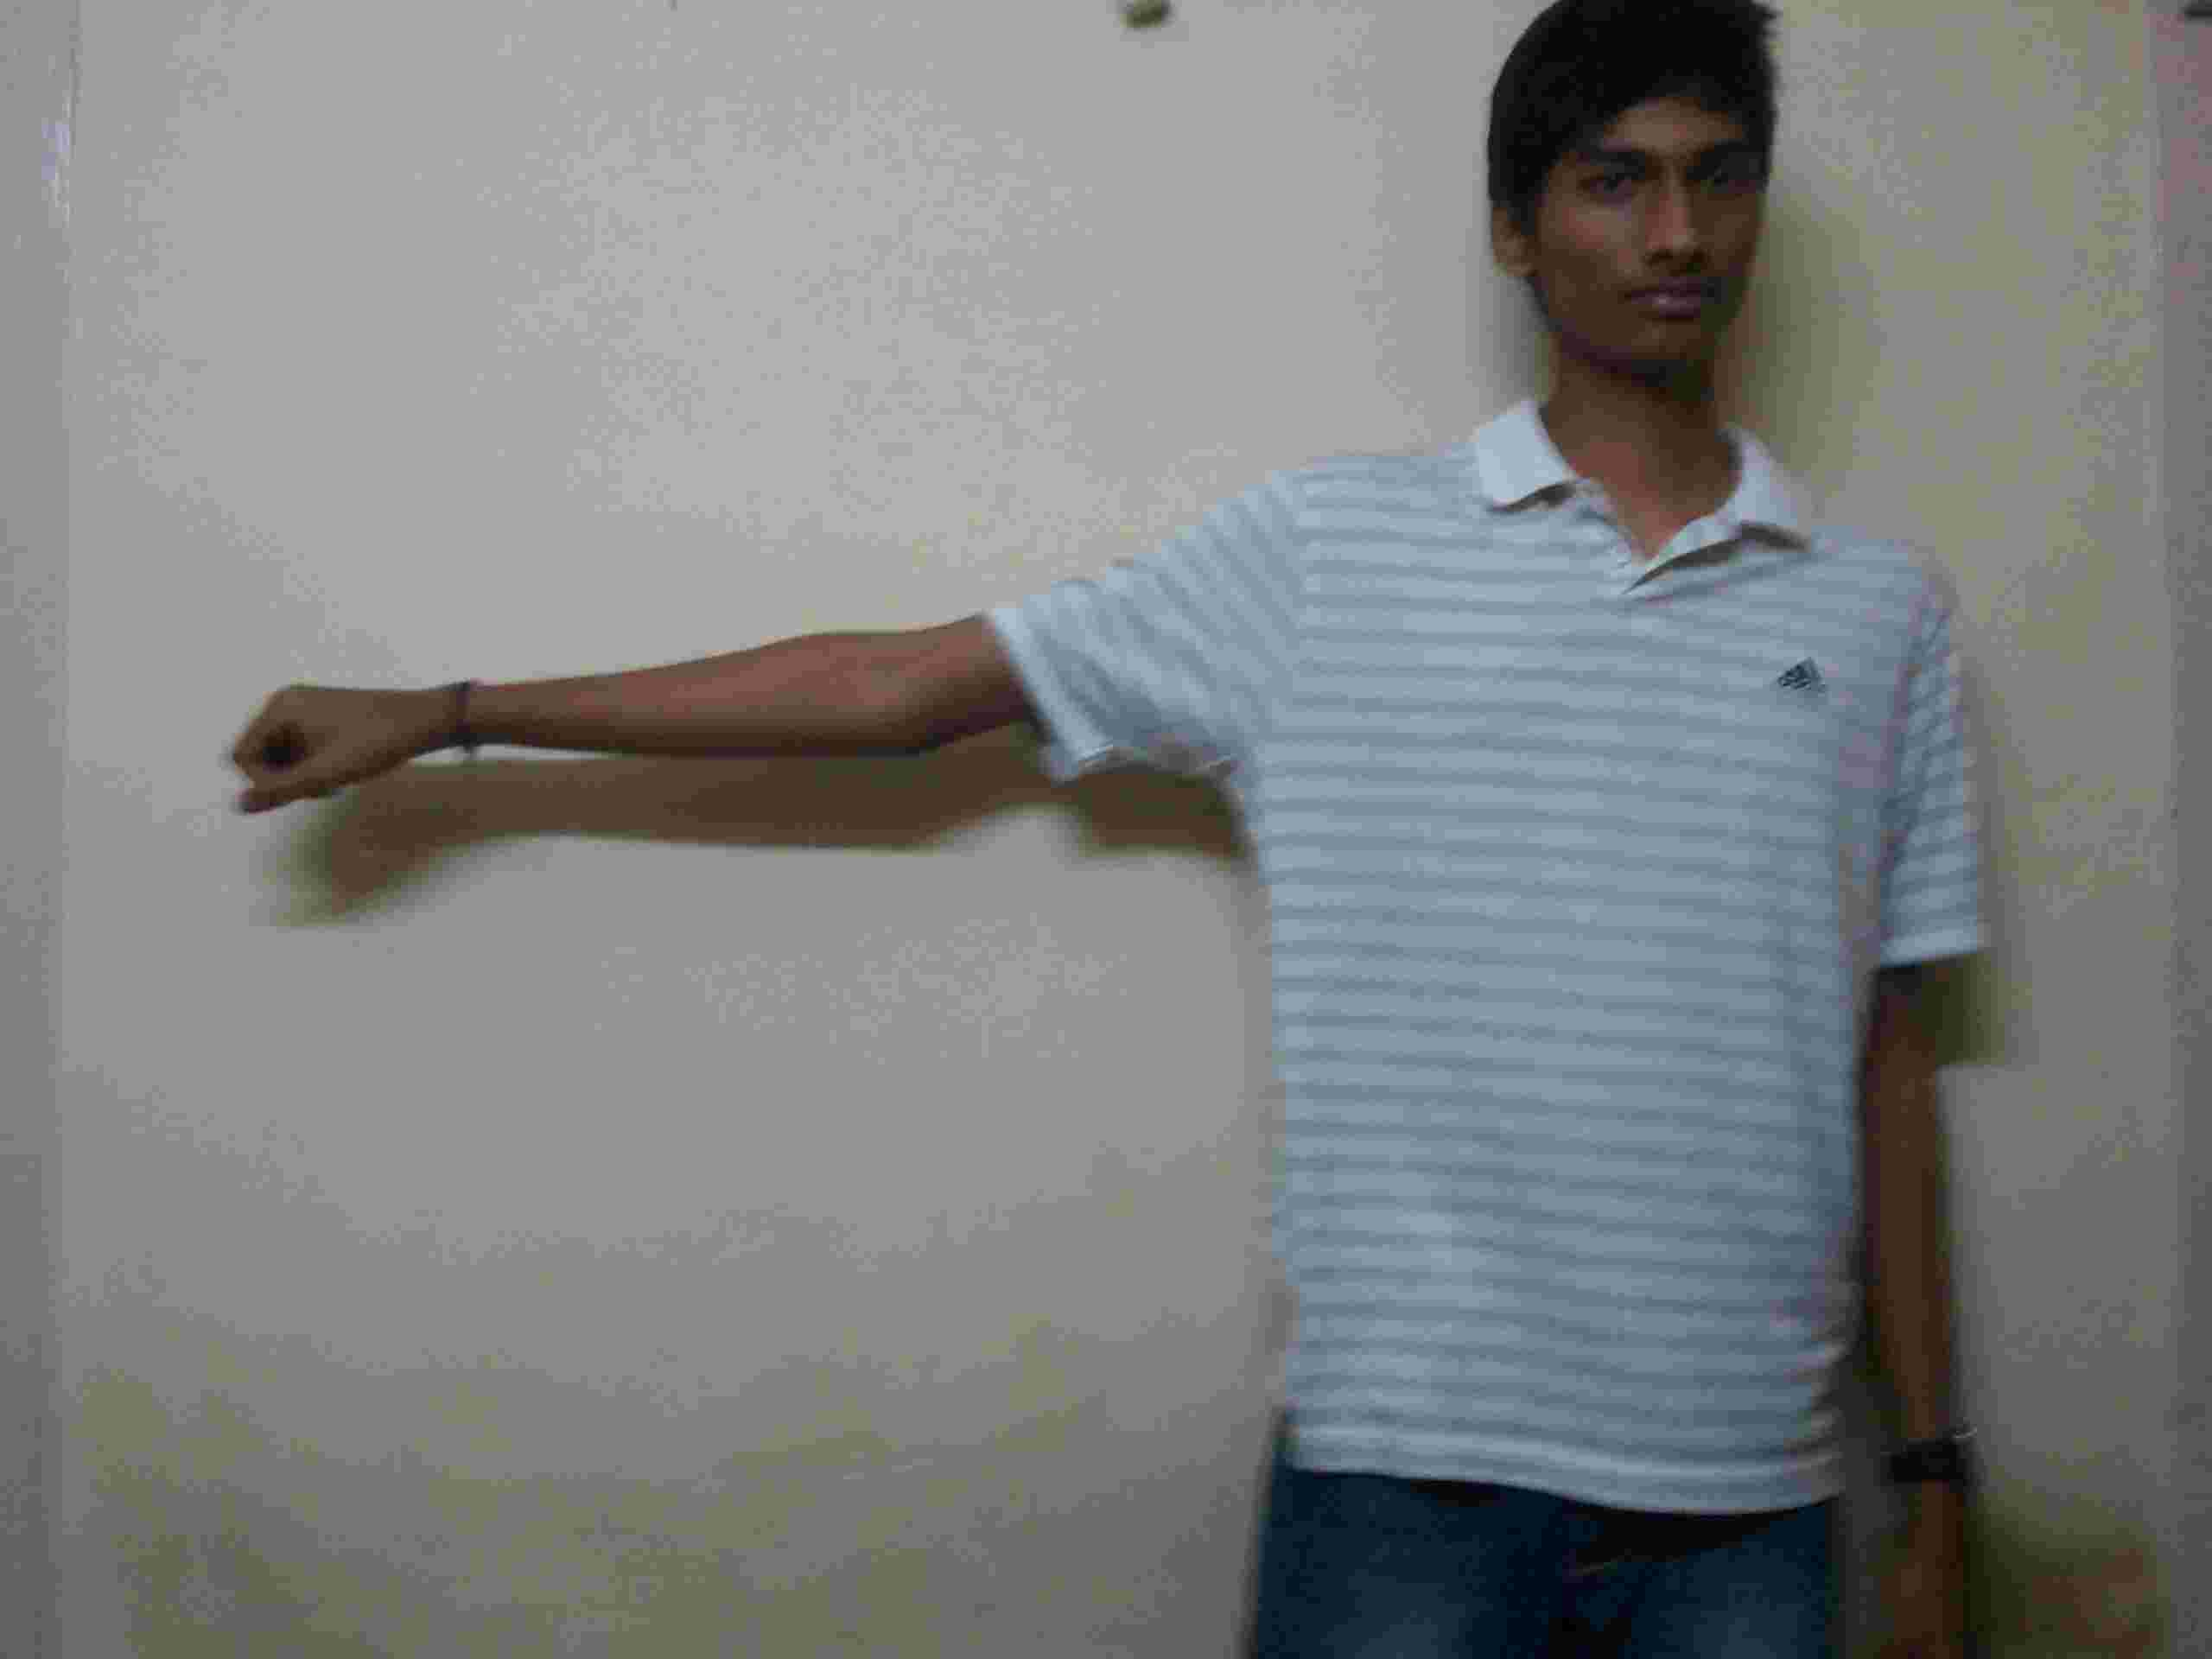
\includegraphics[scale = .08]{gestures/0.jpg} 
  \end{figure}
\end{frame}

\begin{frame}{Hold}
  \begin{figure}
      \centering
      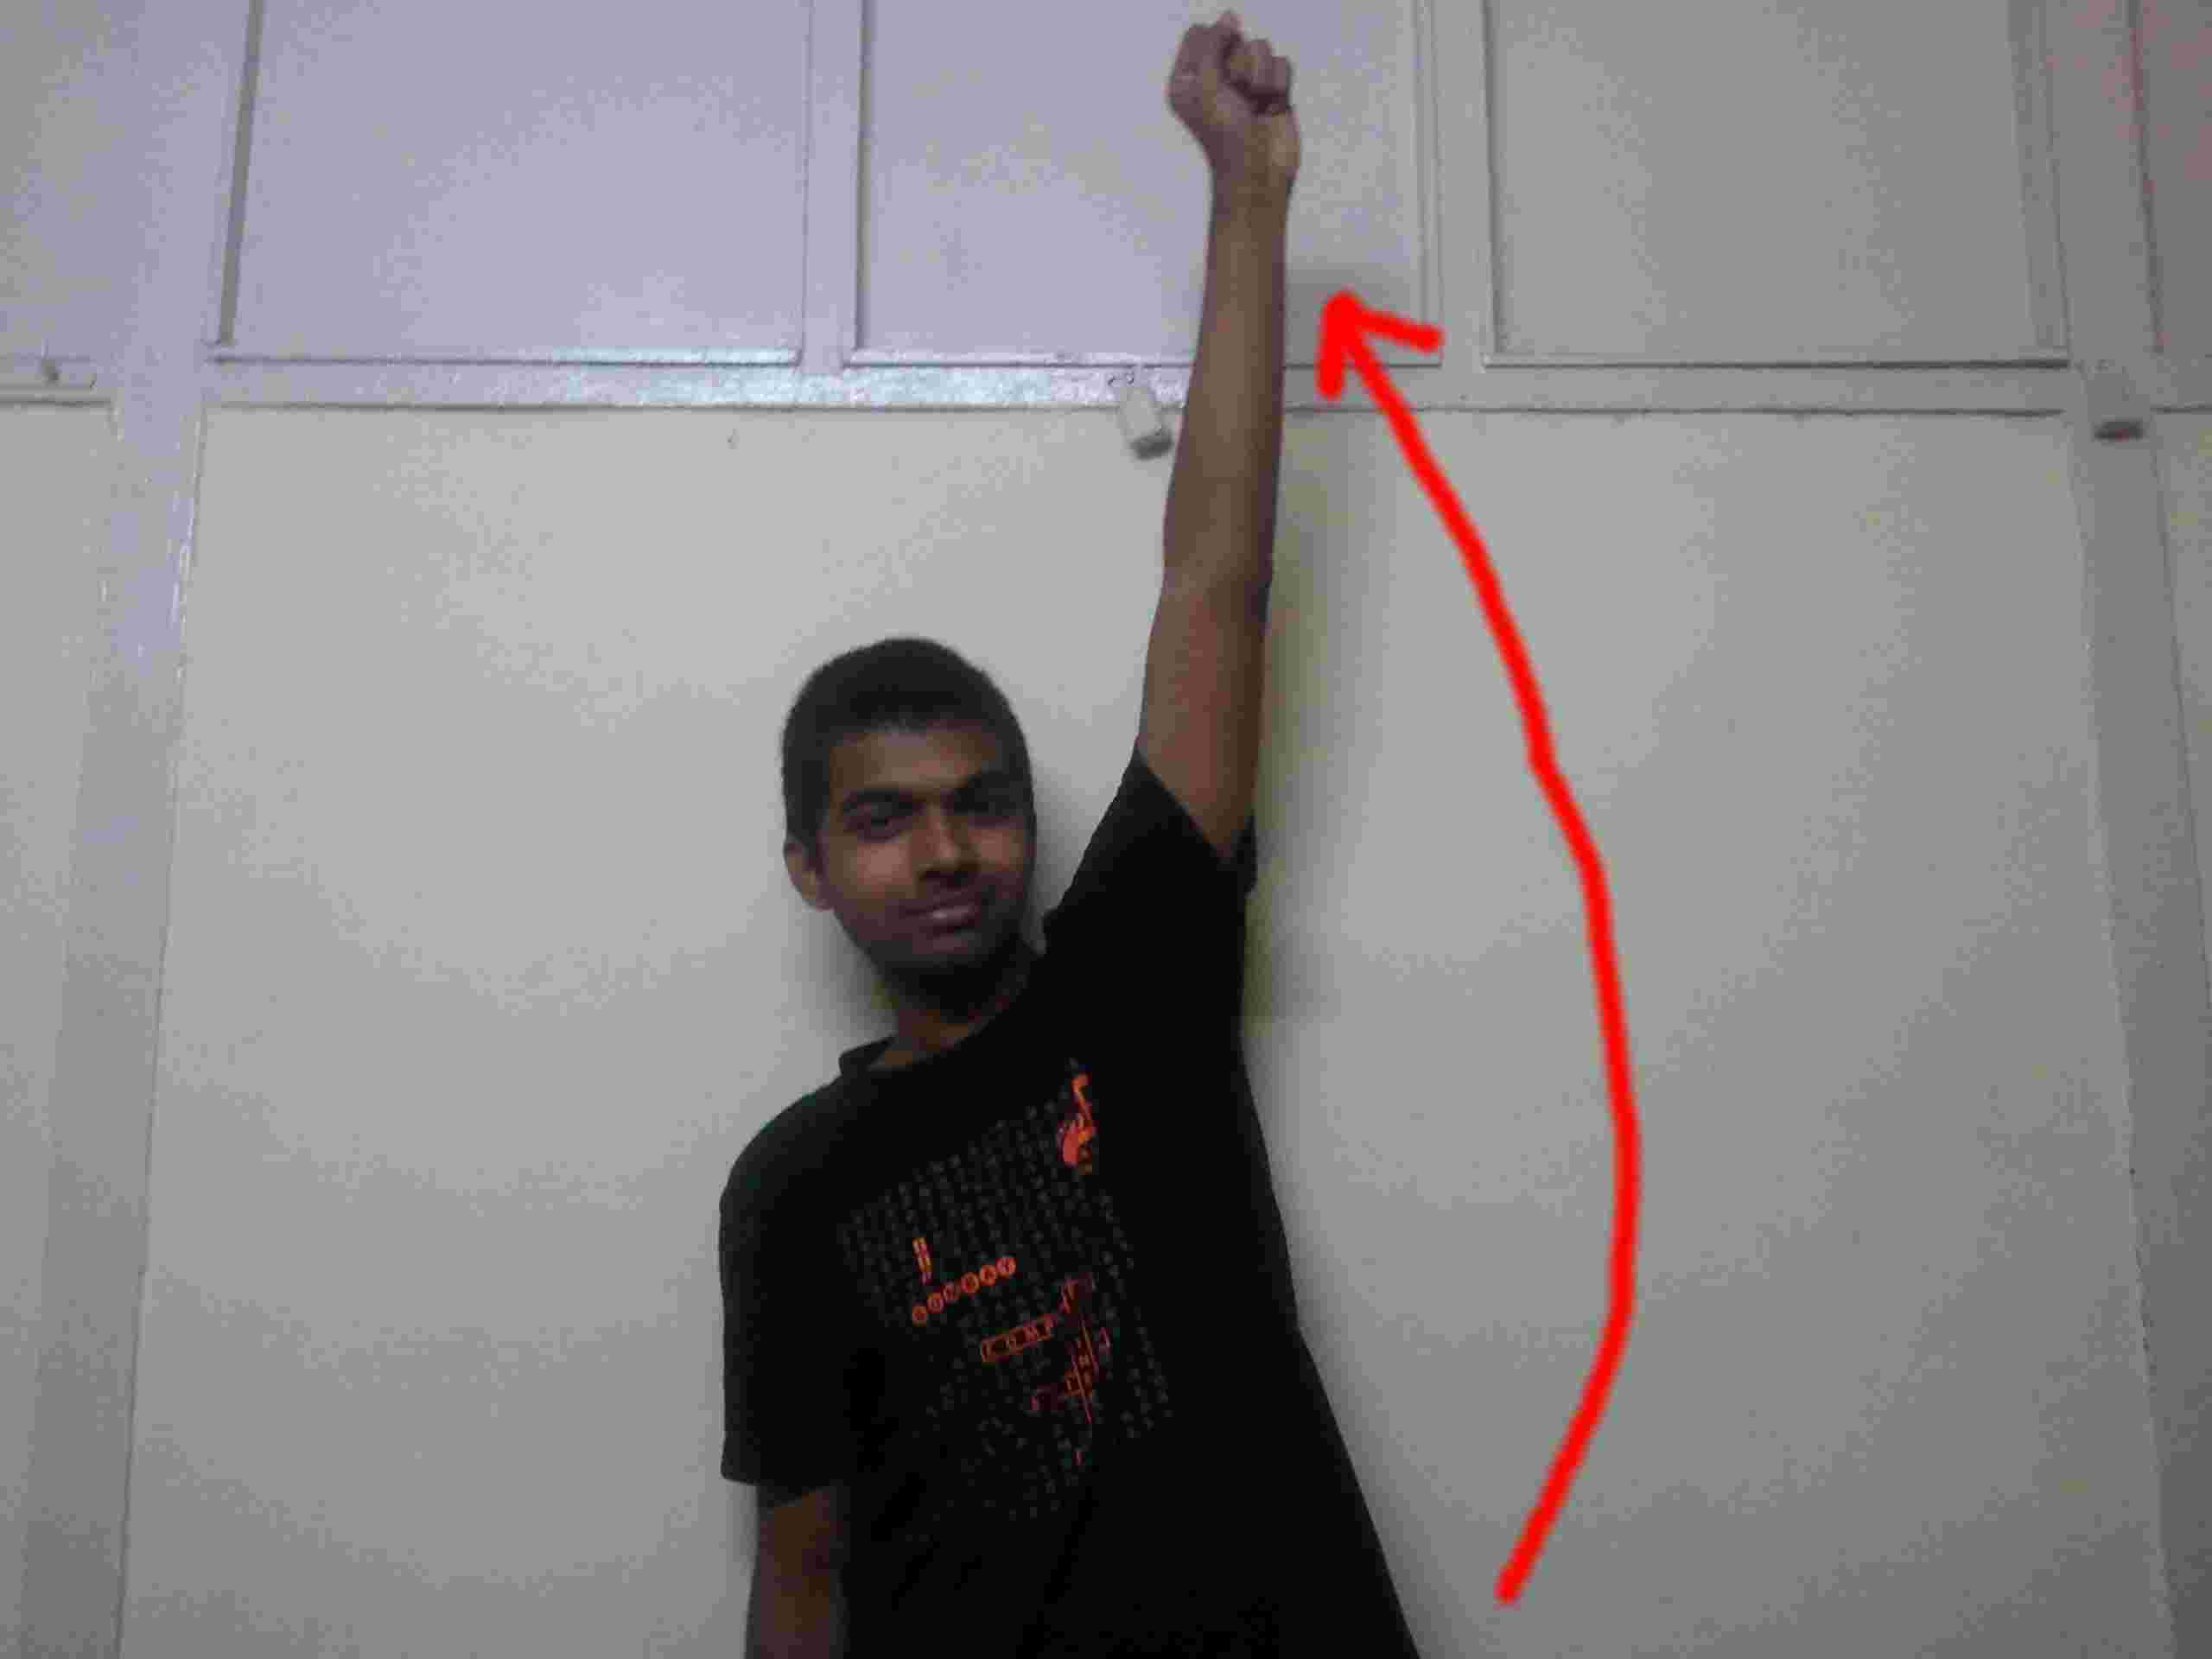
\includegraphics[scale = .08]{gestures/hold.jpg} 
  \end{figure}
\end{frame}

\begin{frame}{1.Base Rotation}
  \begin{figure}
      \centering
      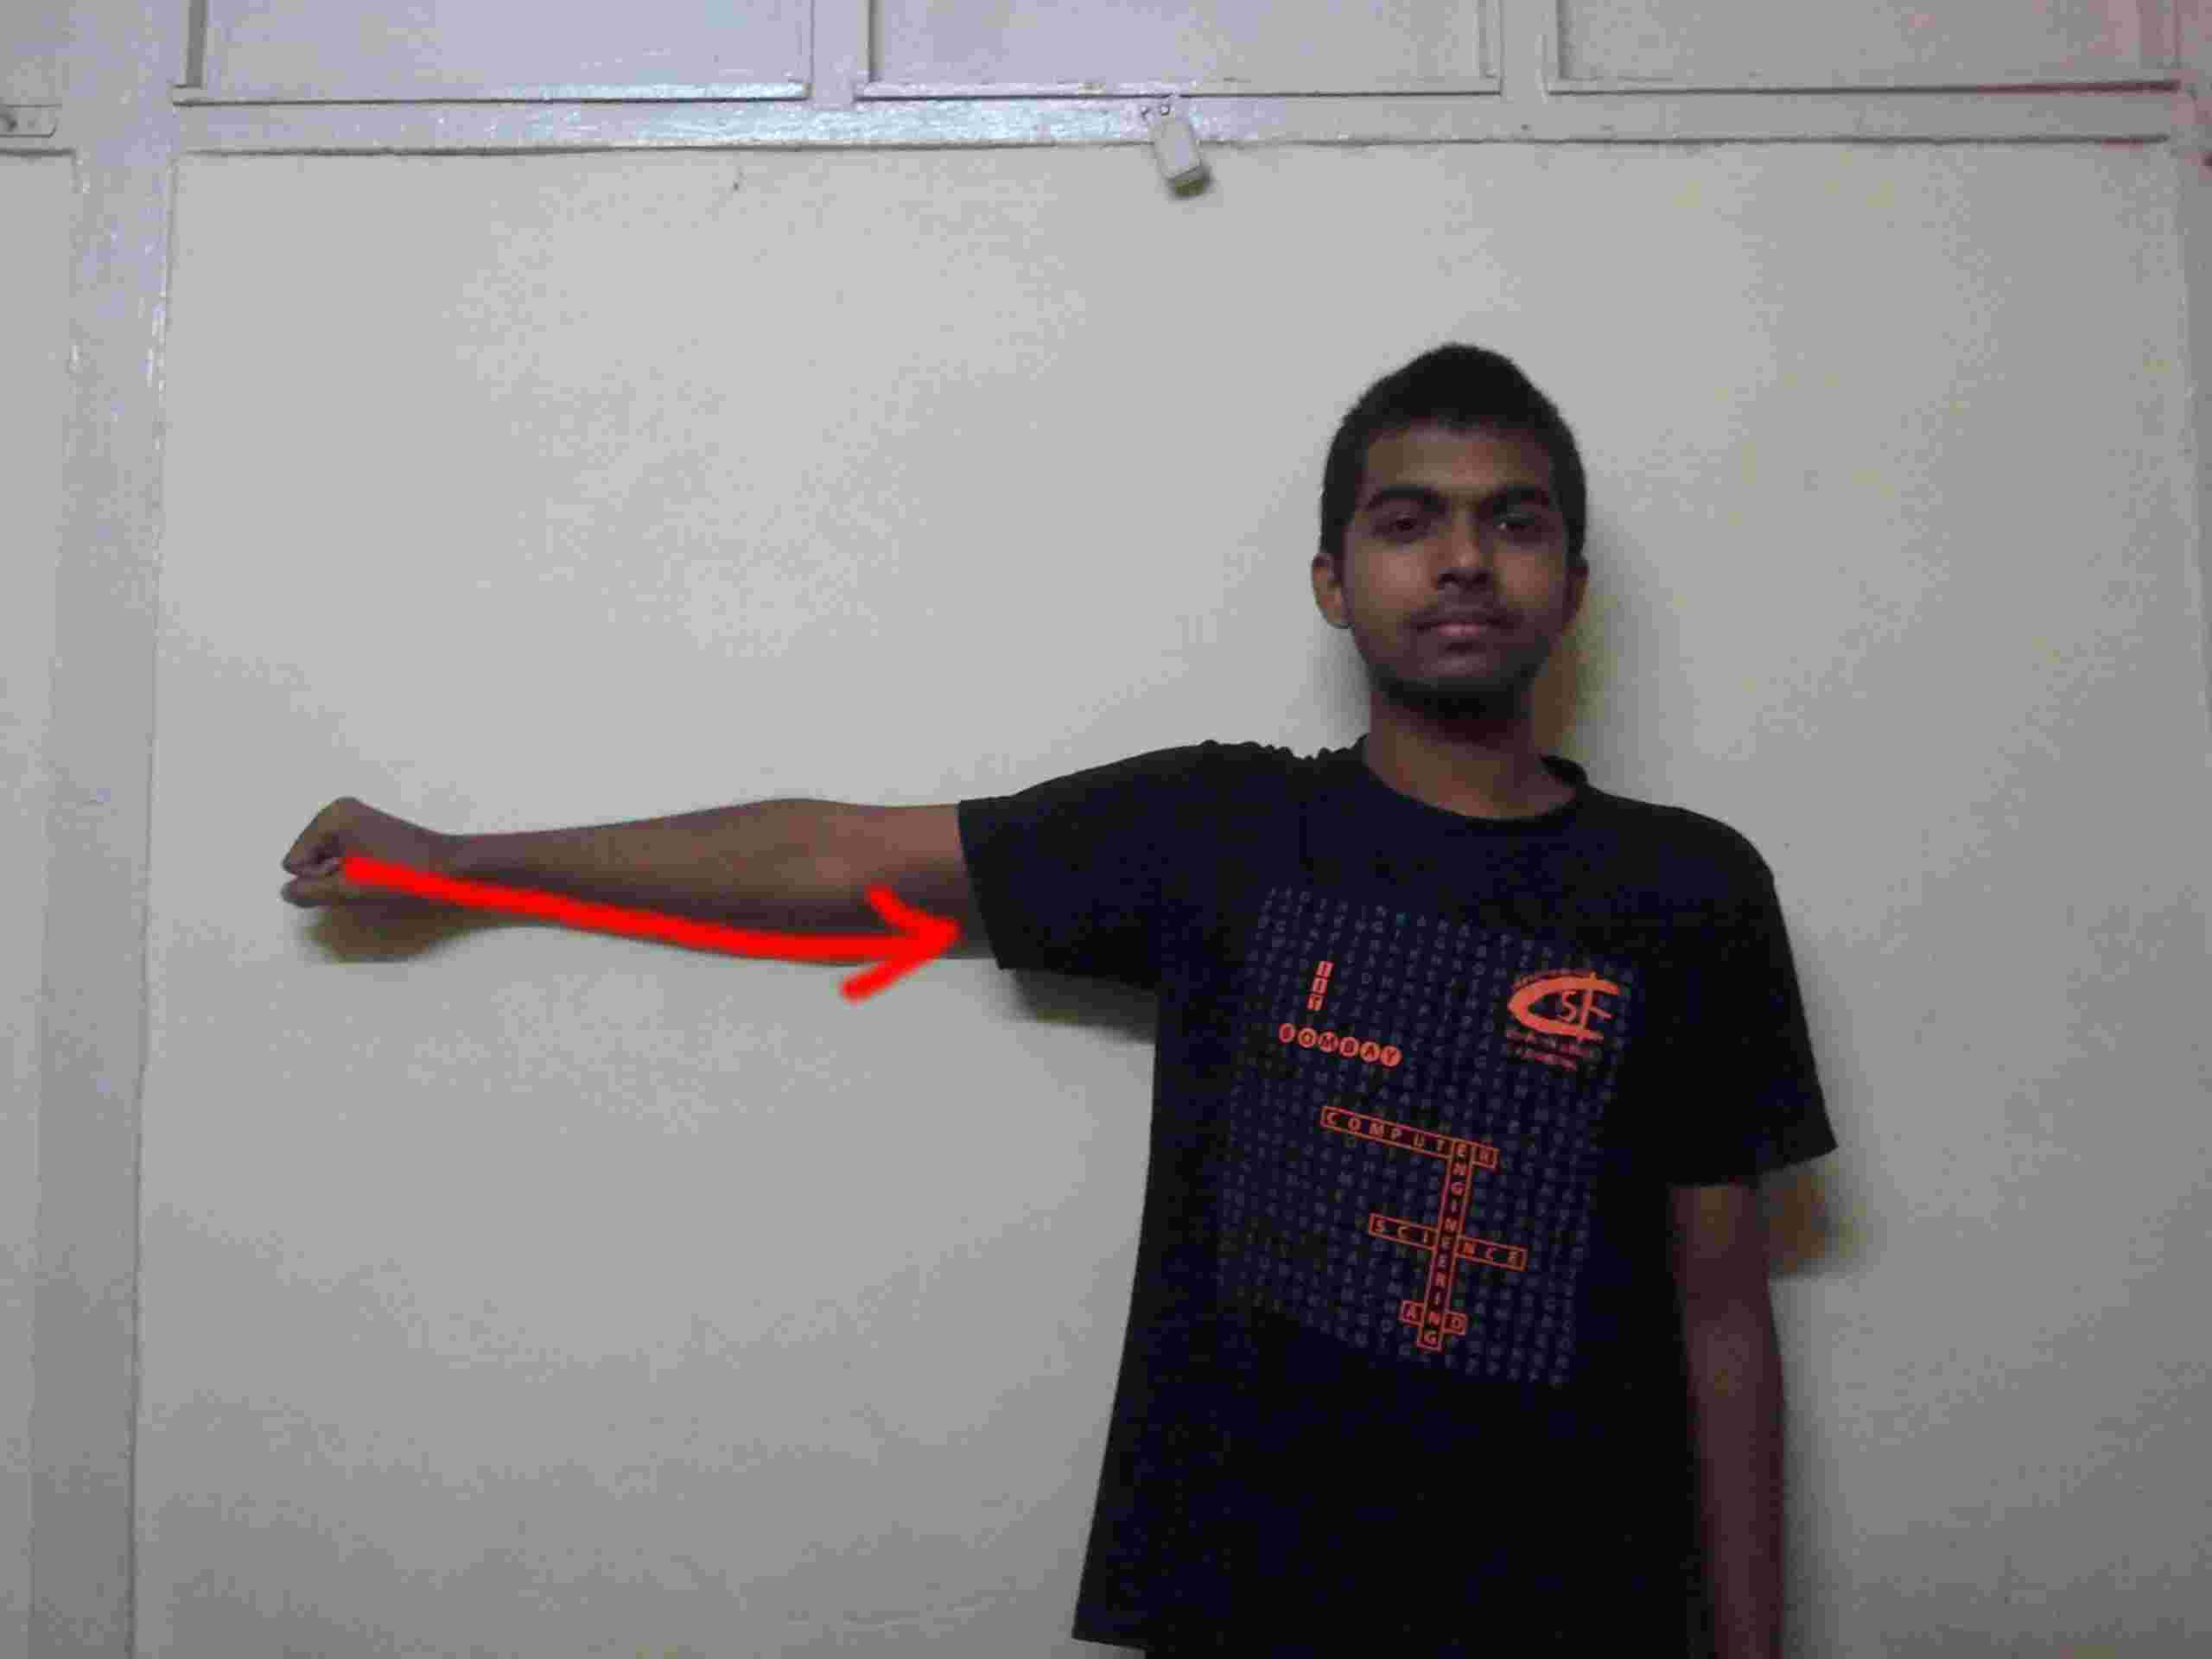
\includegraphics[scale = .06]{gestures/11.jpg} 
      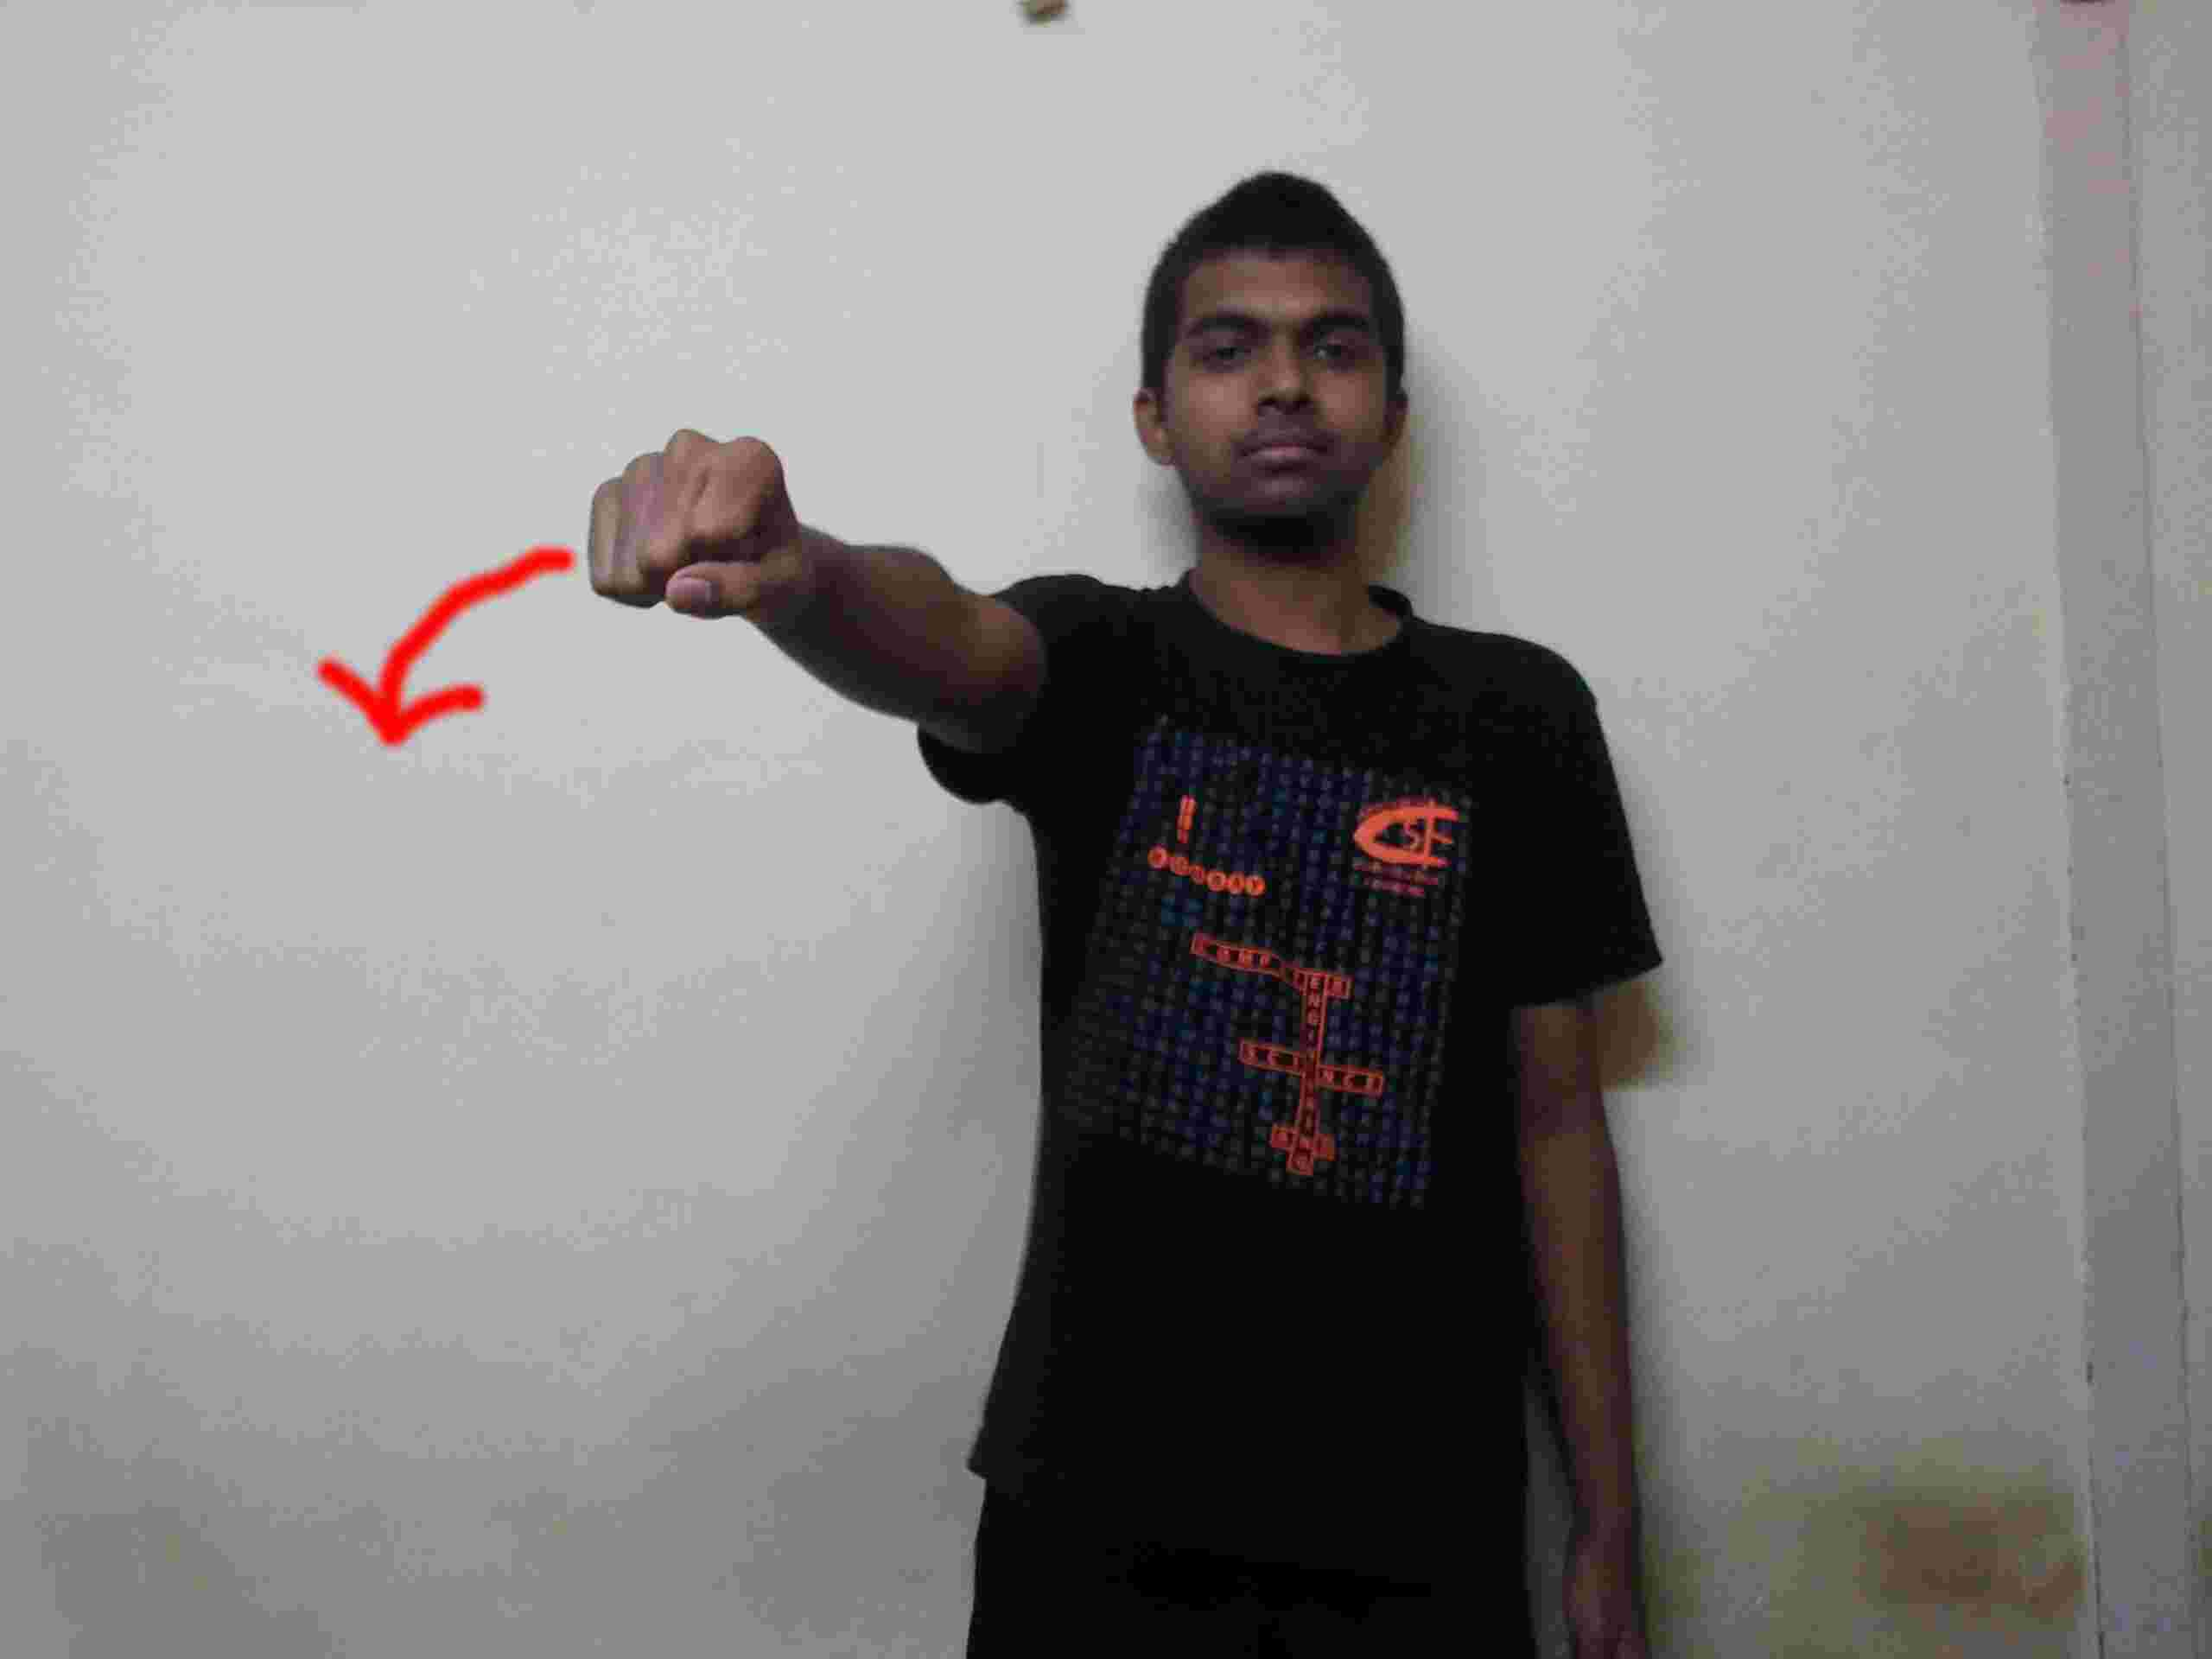
\includegraphics[scale = .06]{gestures/12.jpg} 
  \end{figure}
\end{frame}

\begin{frame}{2.Shoulder Rotation}
  \begin{figure}
      \centering
      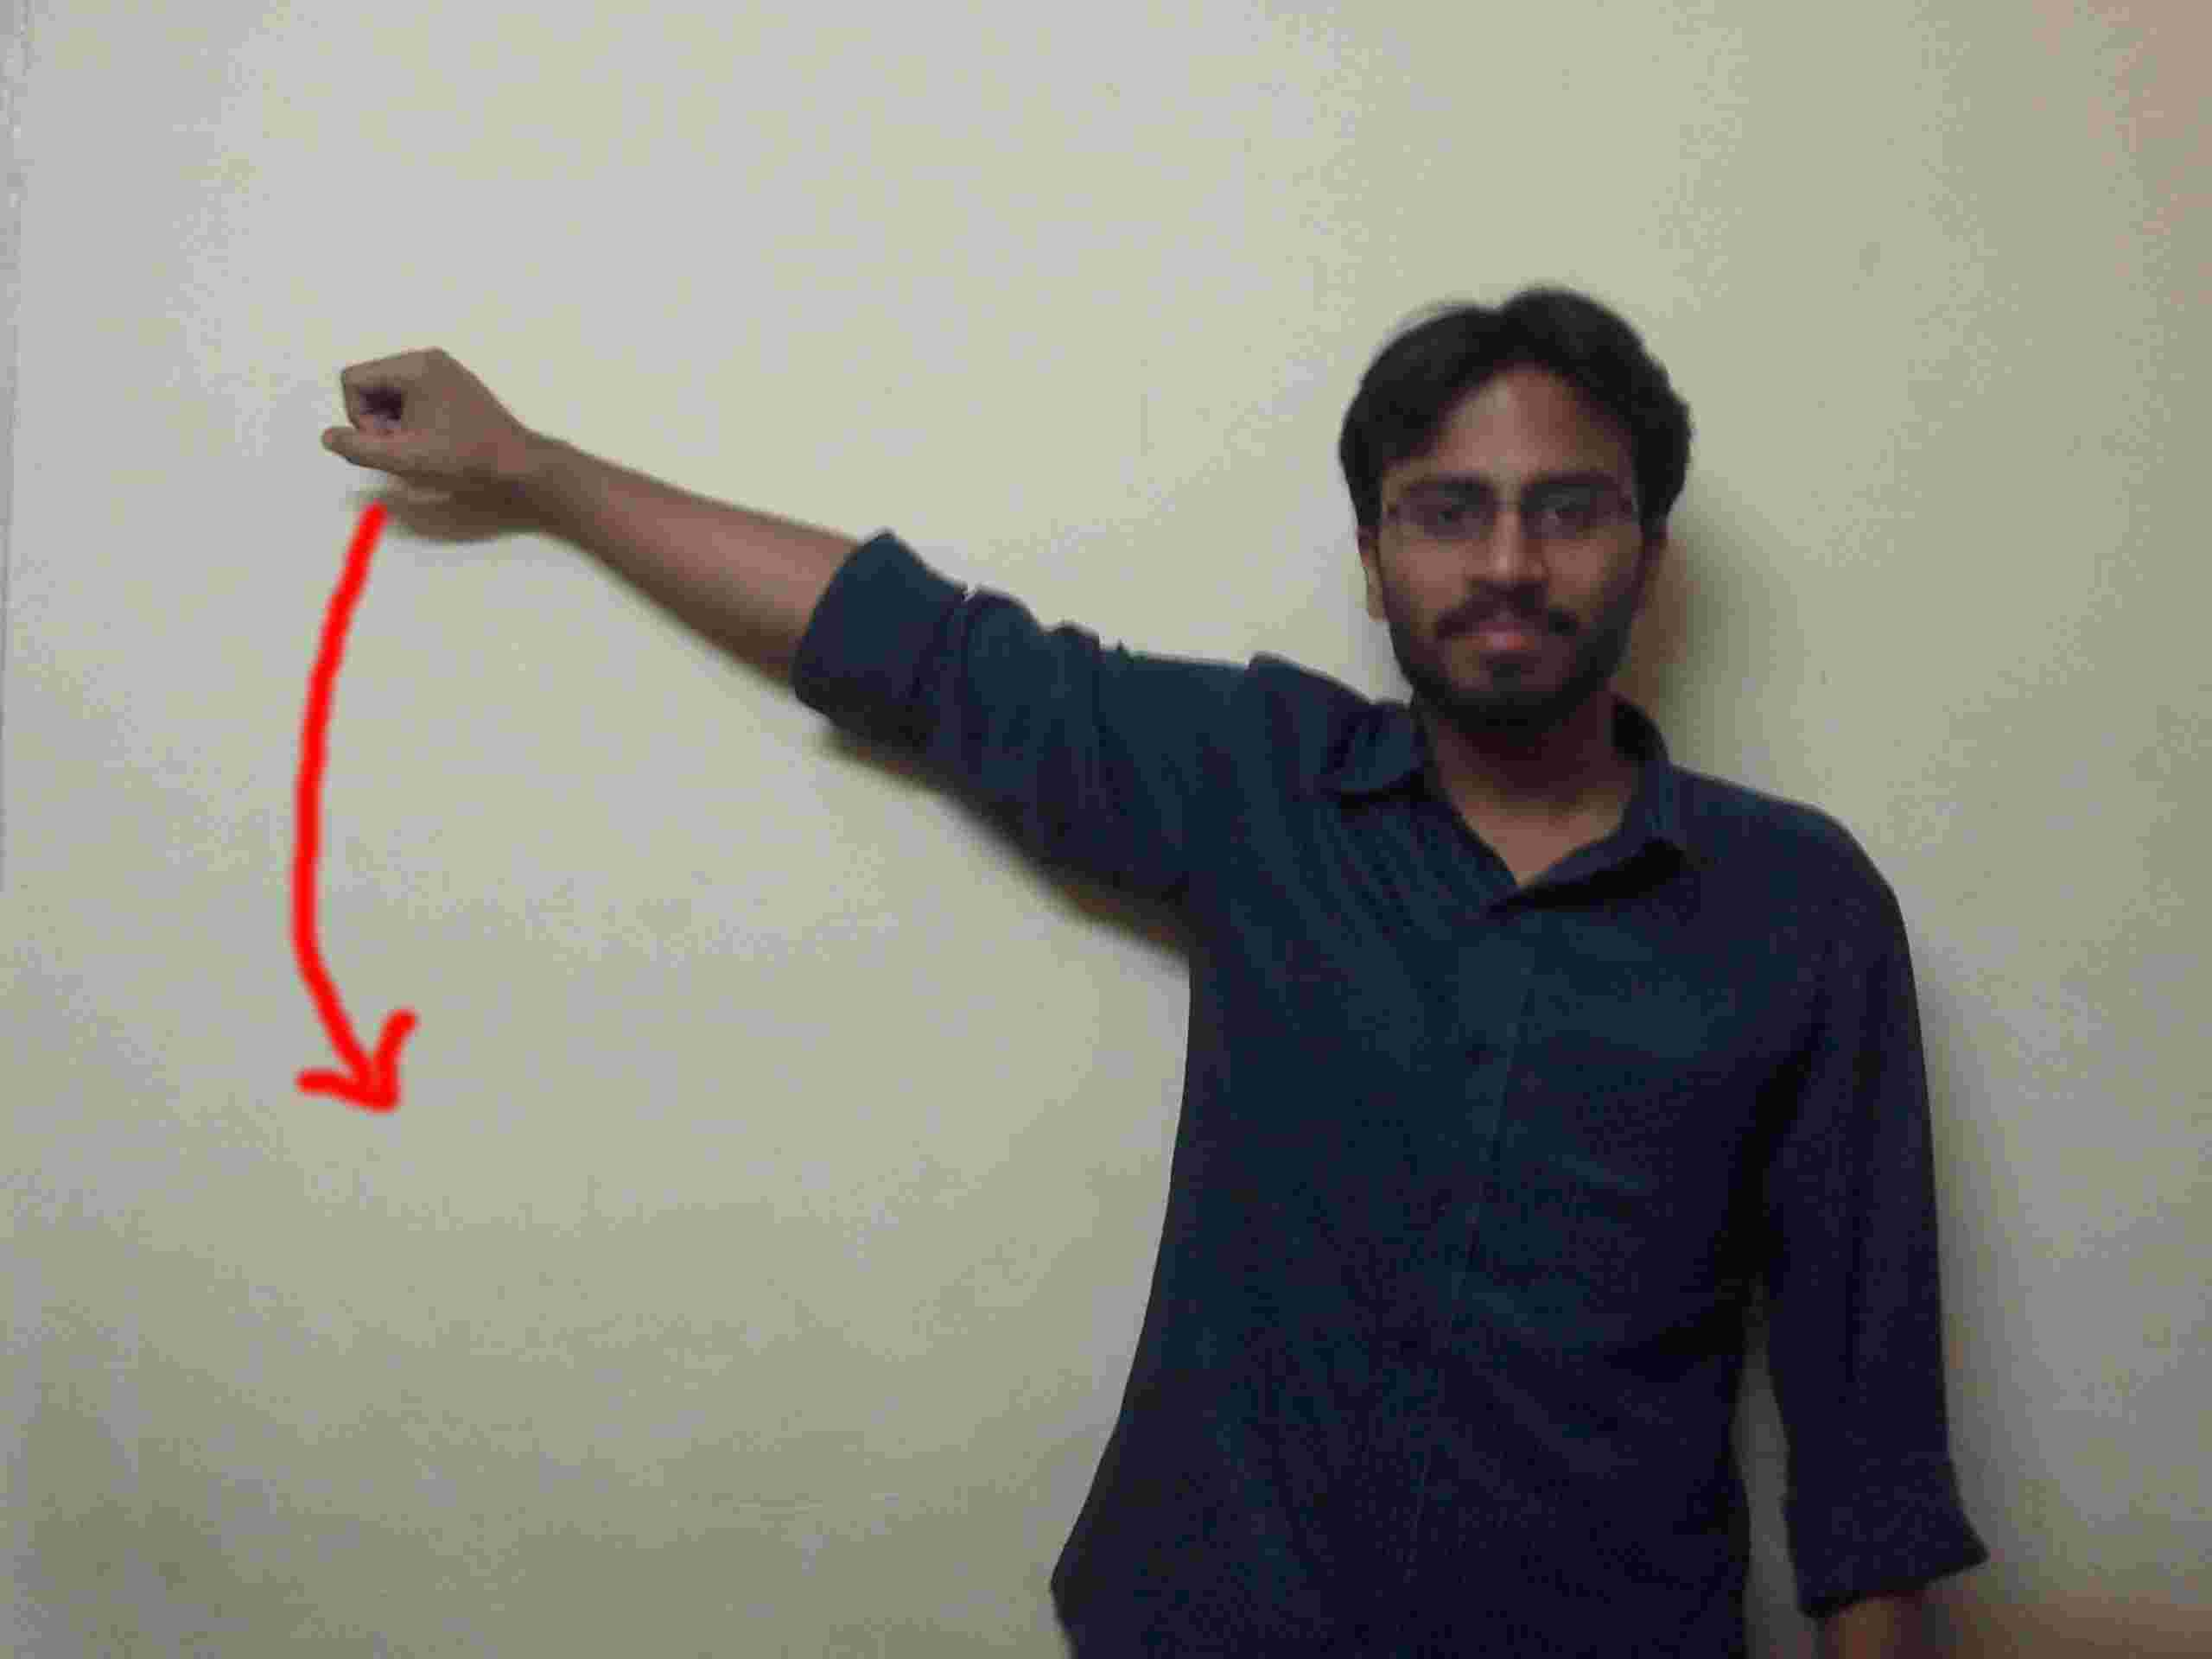
\includegraphics[scale = .06]{gestures/21.jpg} 
      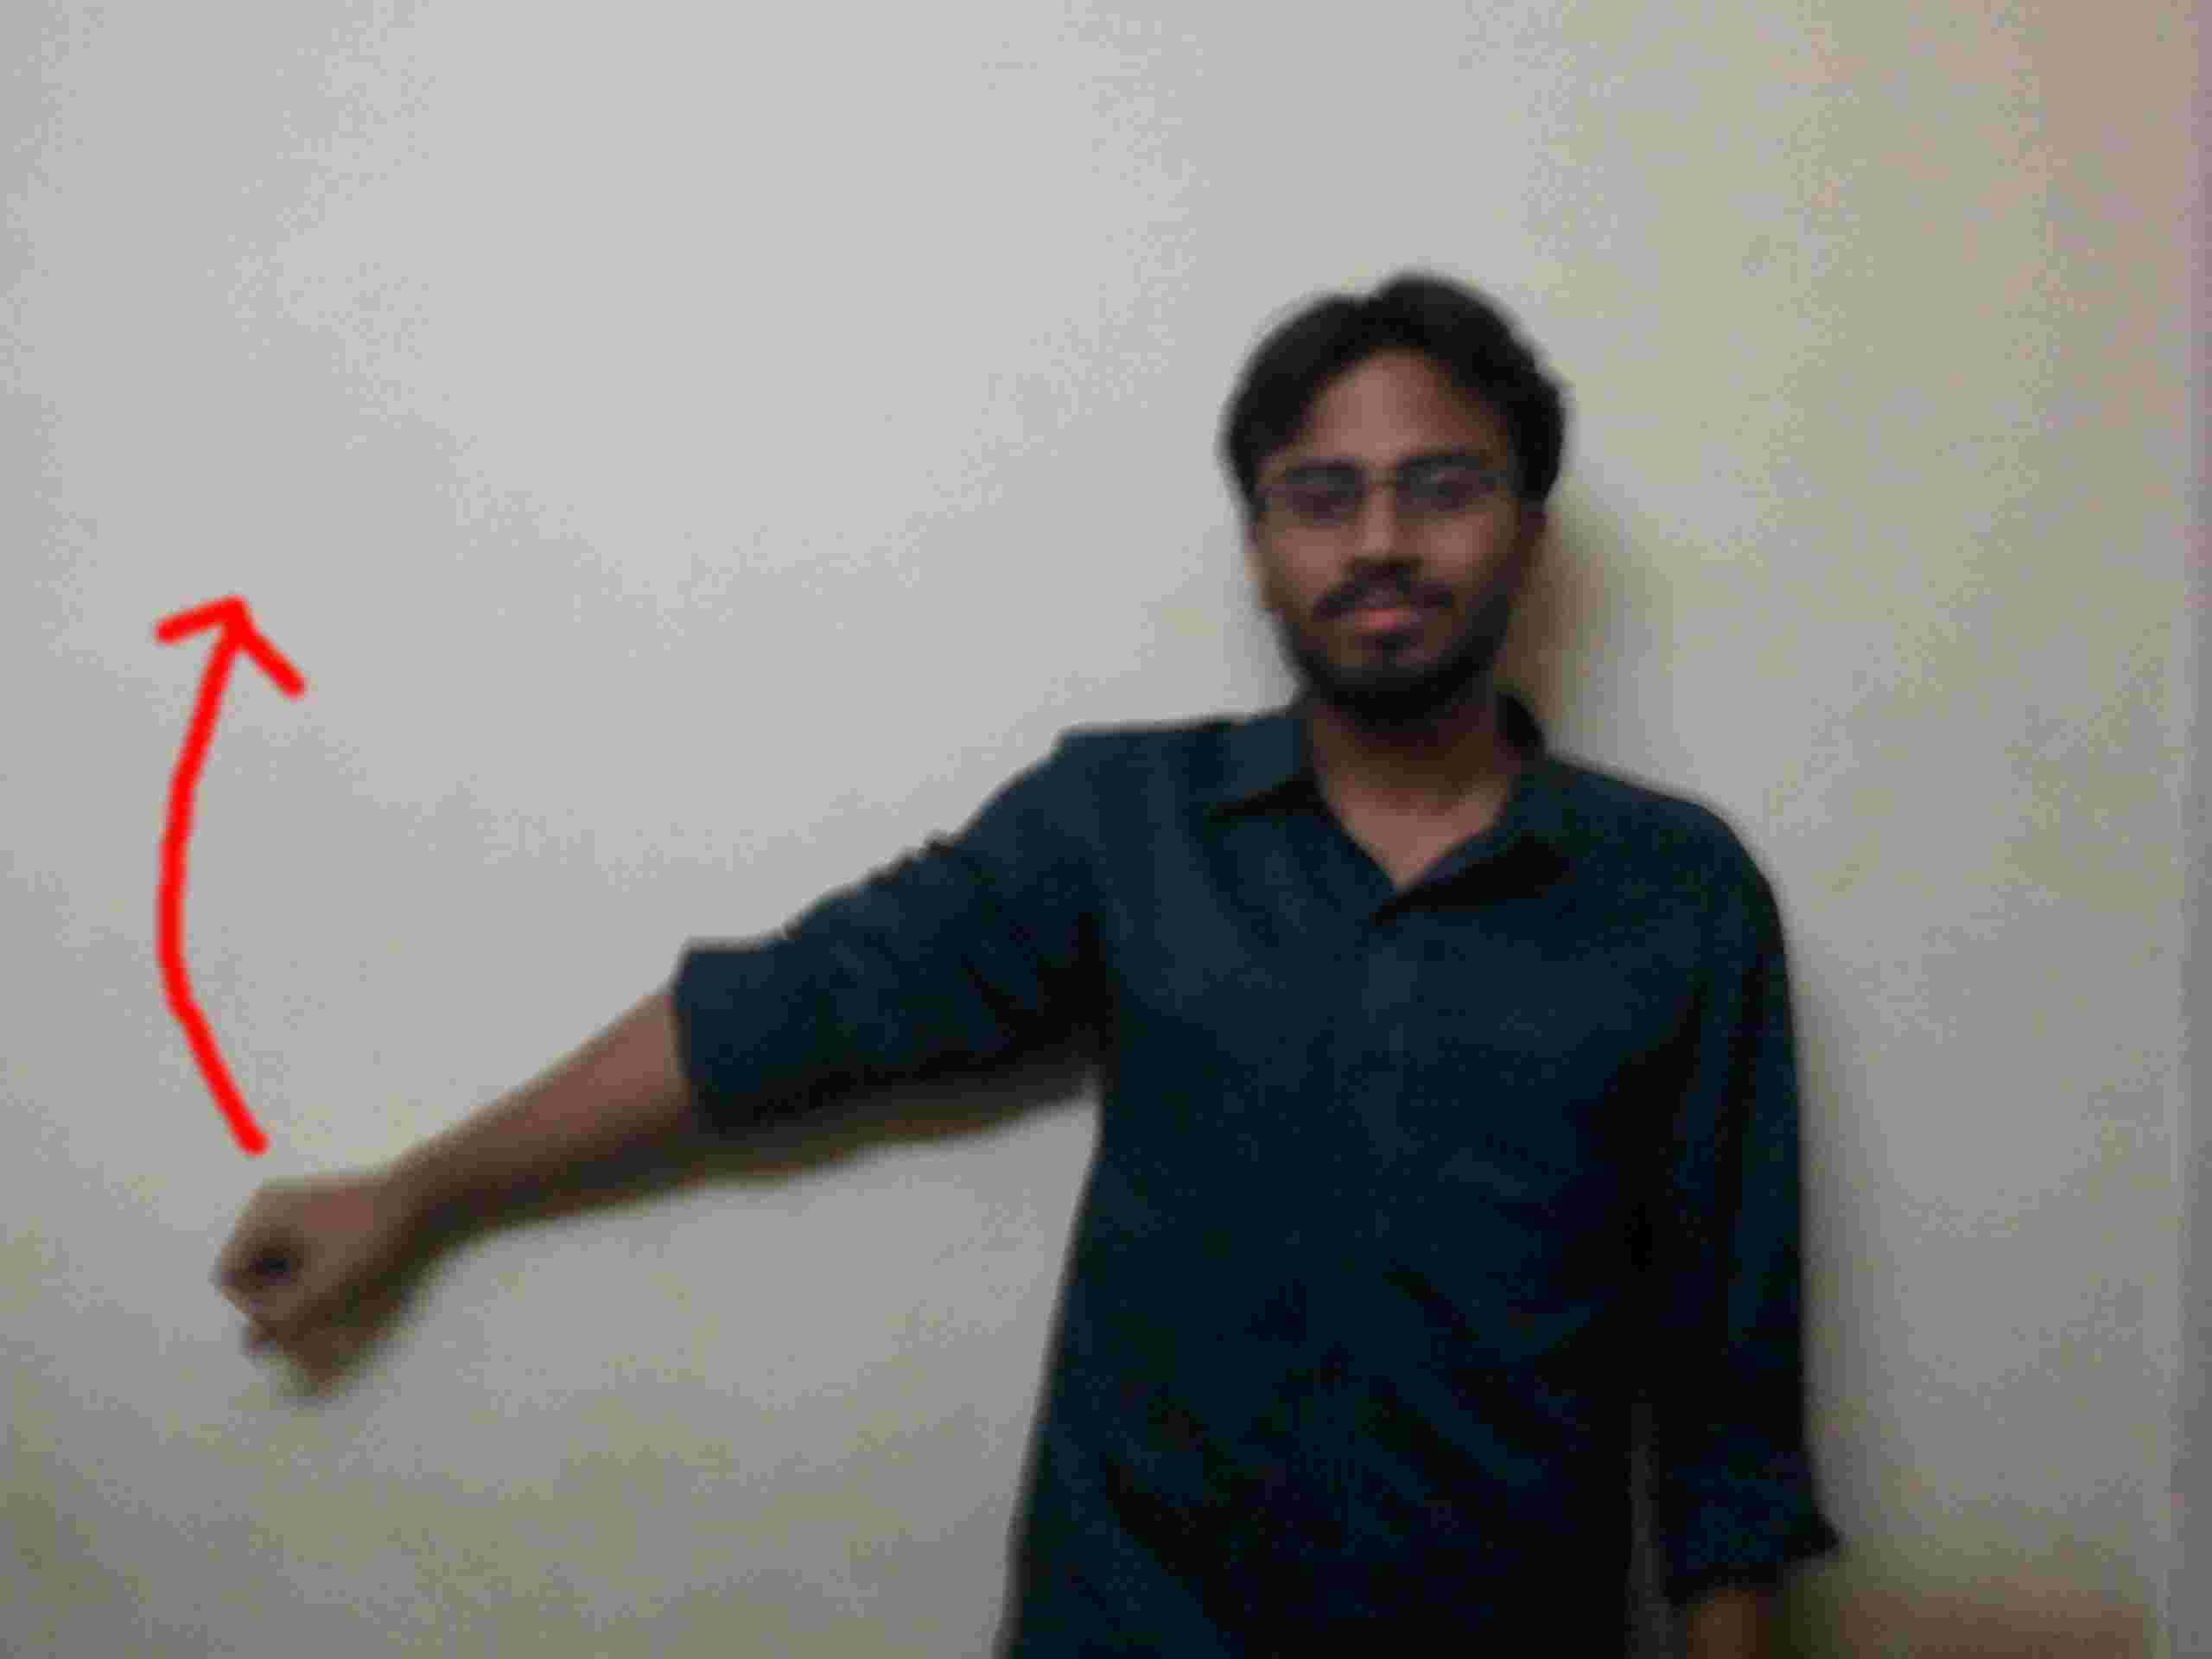
\includegraphics[scale = .06]{gestures/22.jpg} 
  \end{figure}
\end{frame}

\begin{frame}{3.Elbow Rotation}
  \begin{figure}
      \centering
      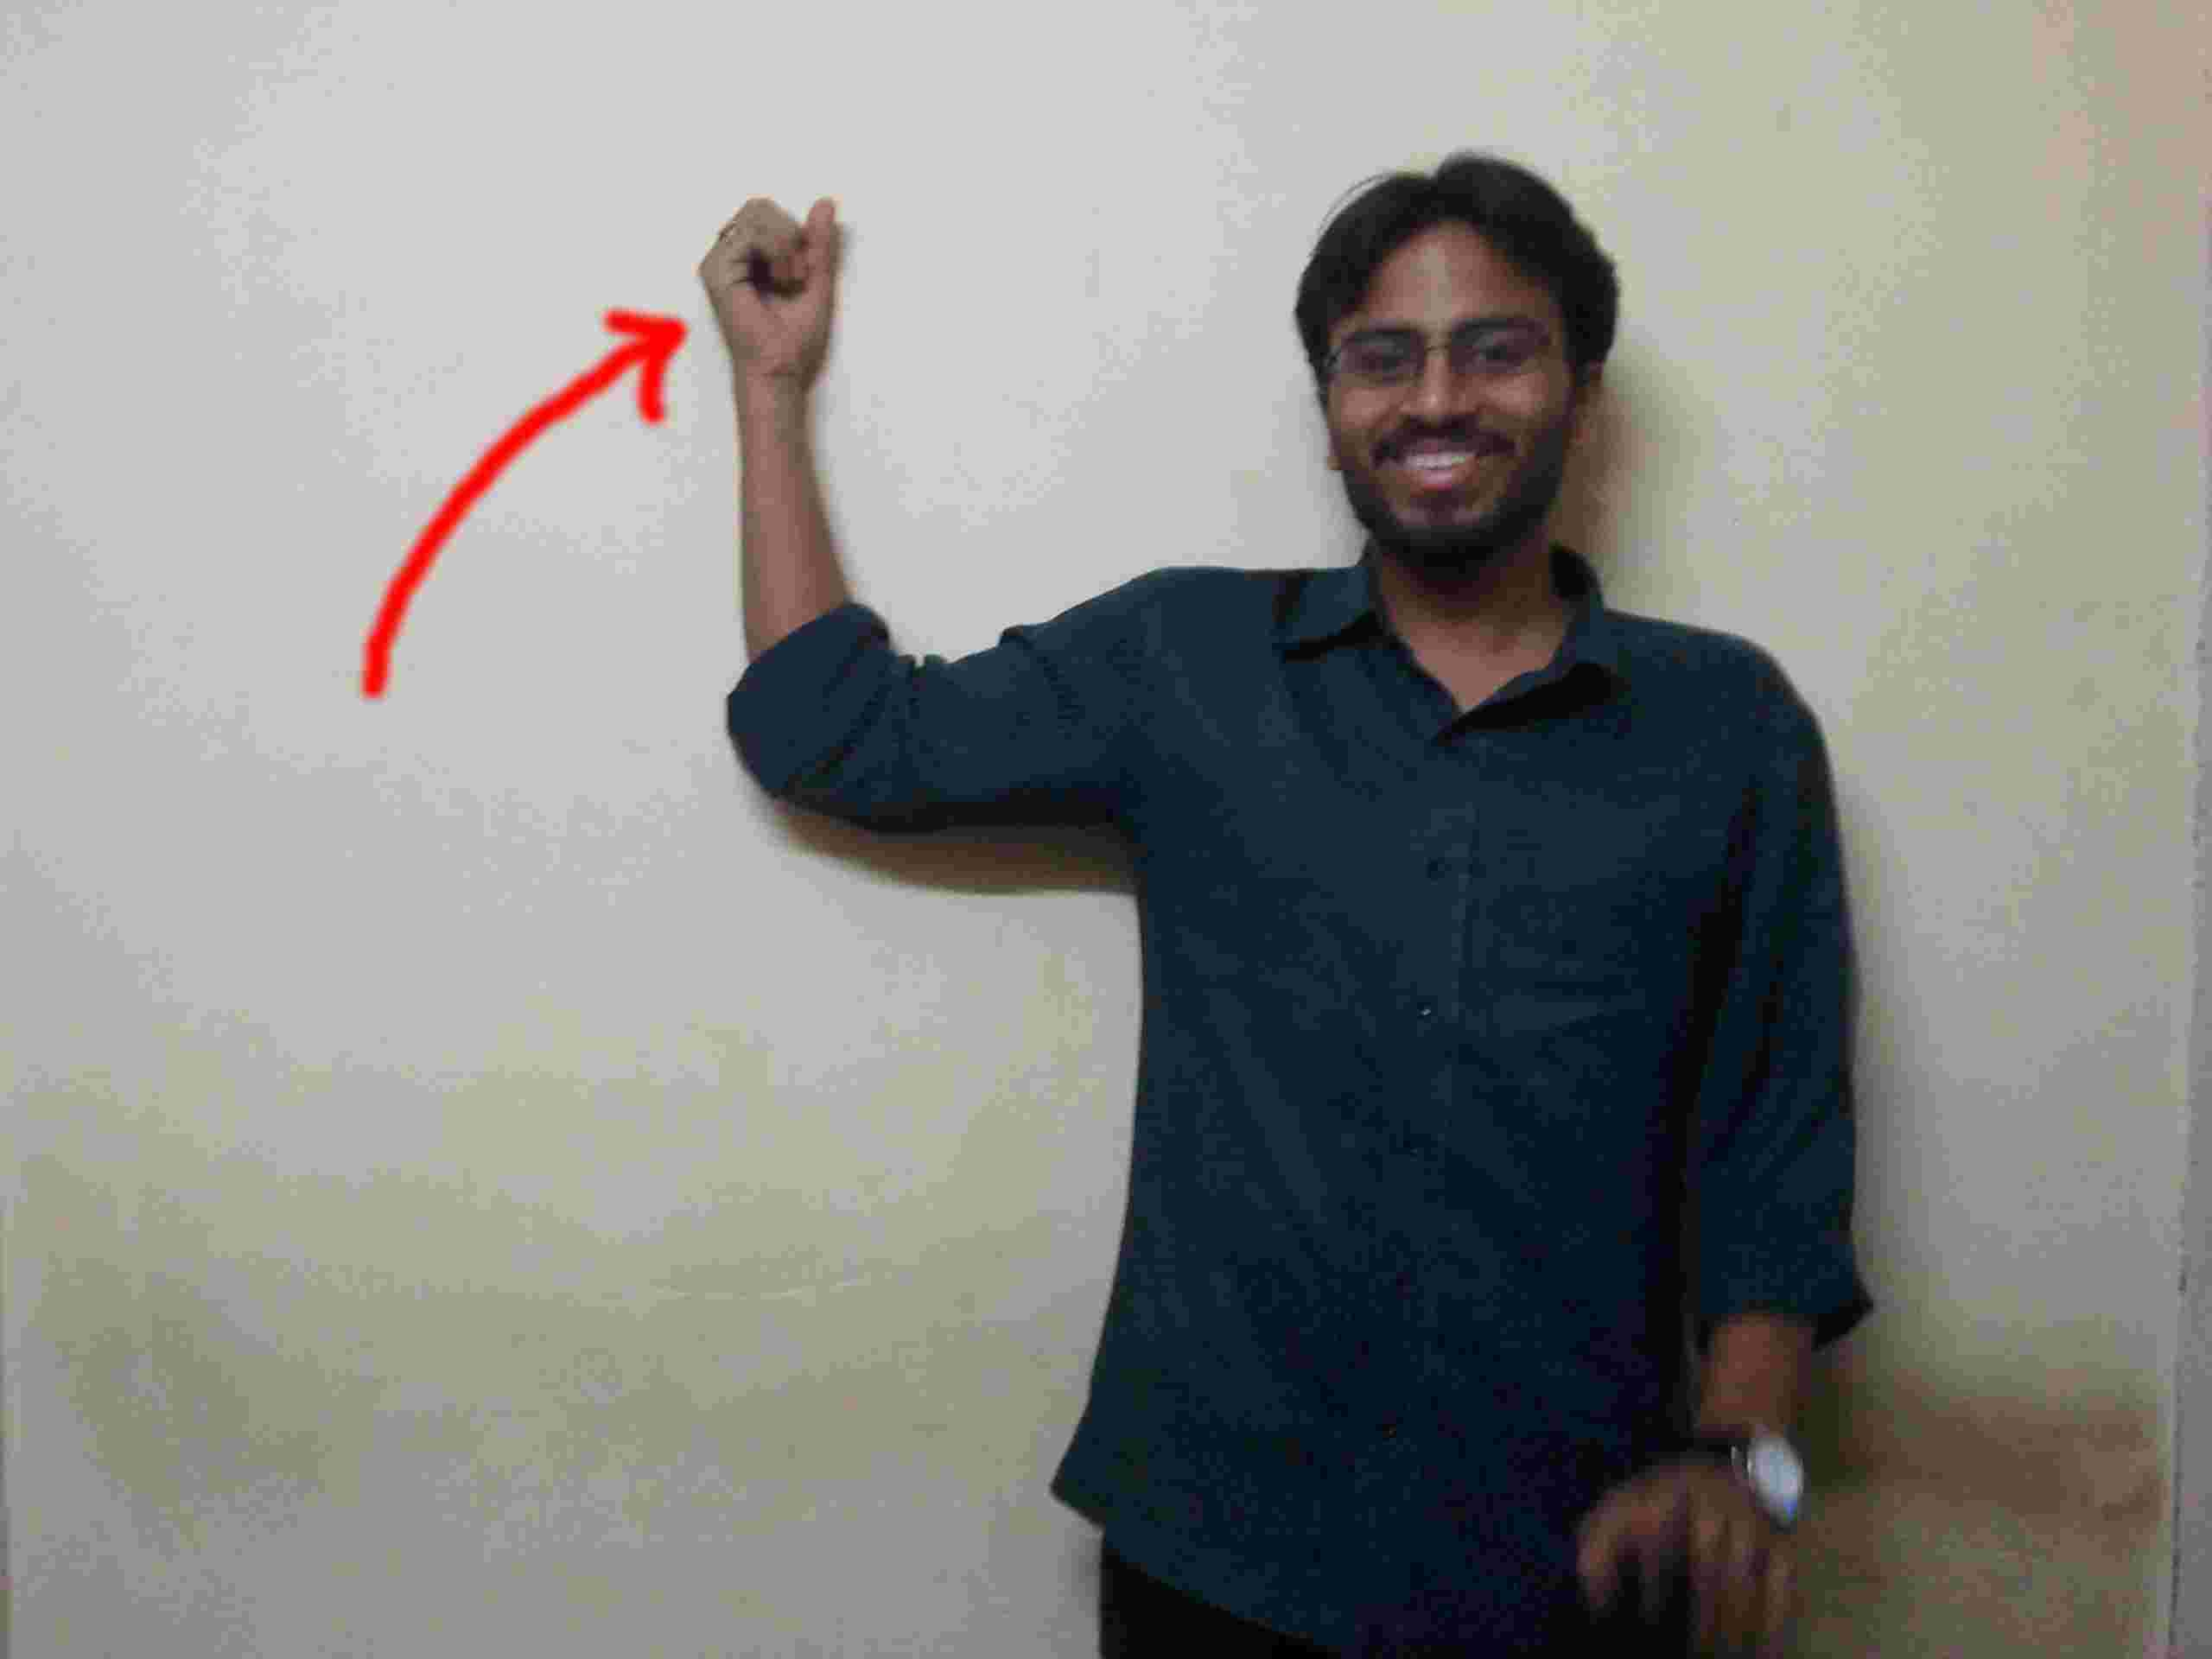
\includegraphics[scale = .06]{gestures/31.jpg} 
      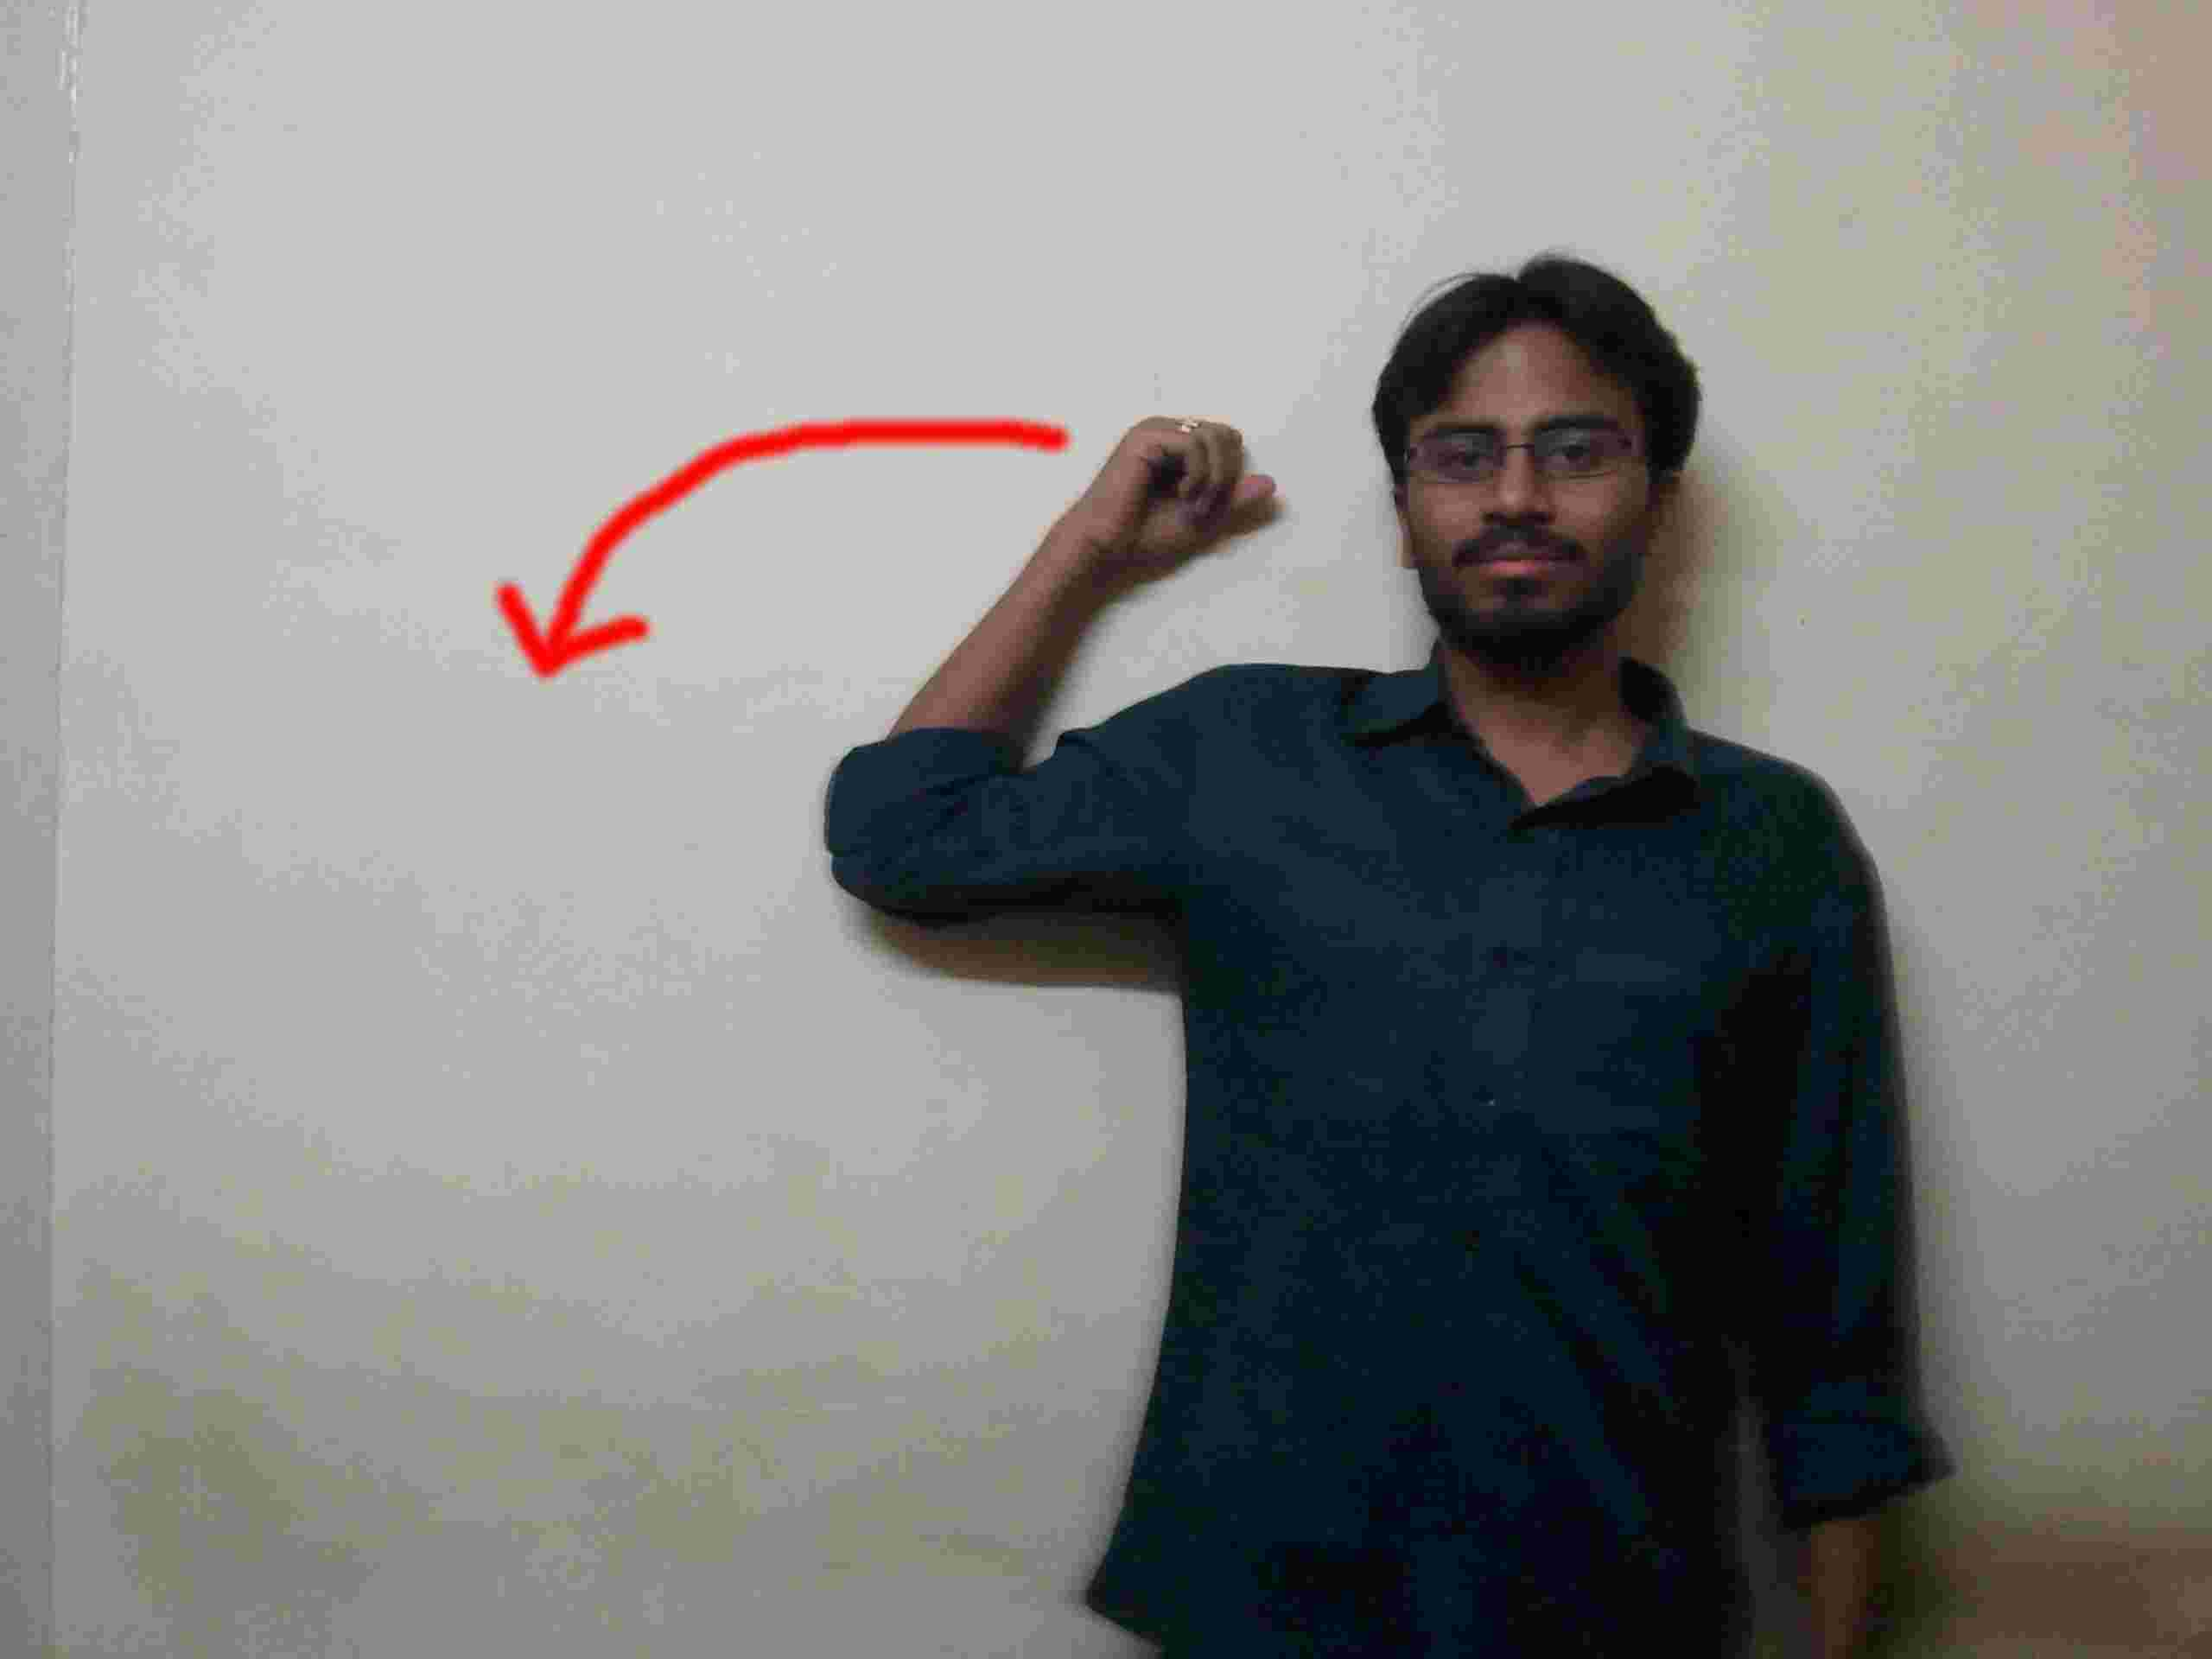
\includegraphics[scale = .06]{gestures/32.jpg} 
  \end{figure}
\end{frame}

\begin{frame}{4.Wrist Pitch}
  \begin{figure}
      \centering
      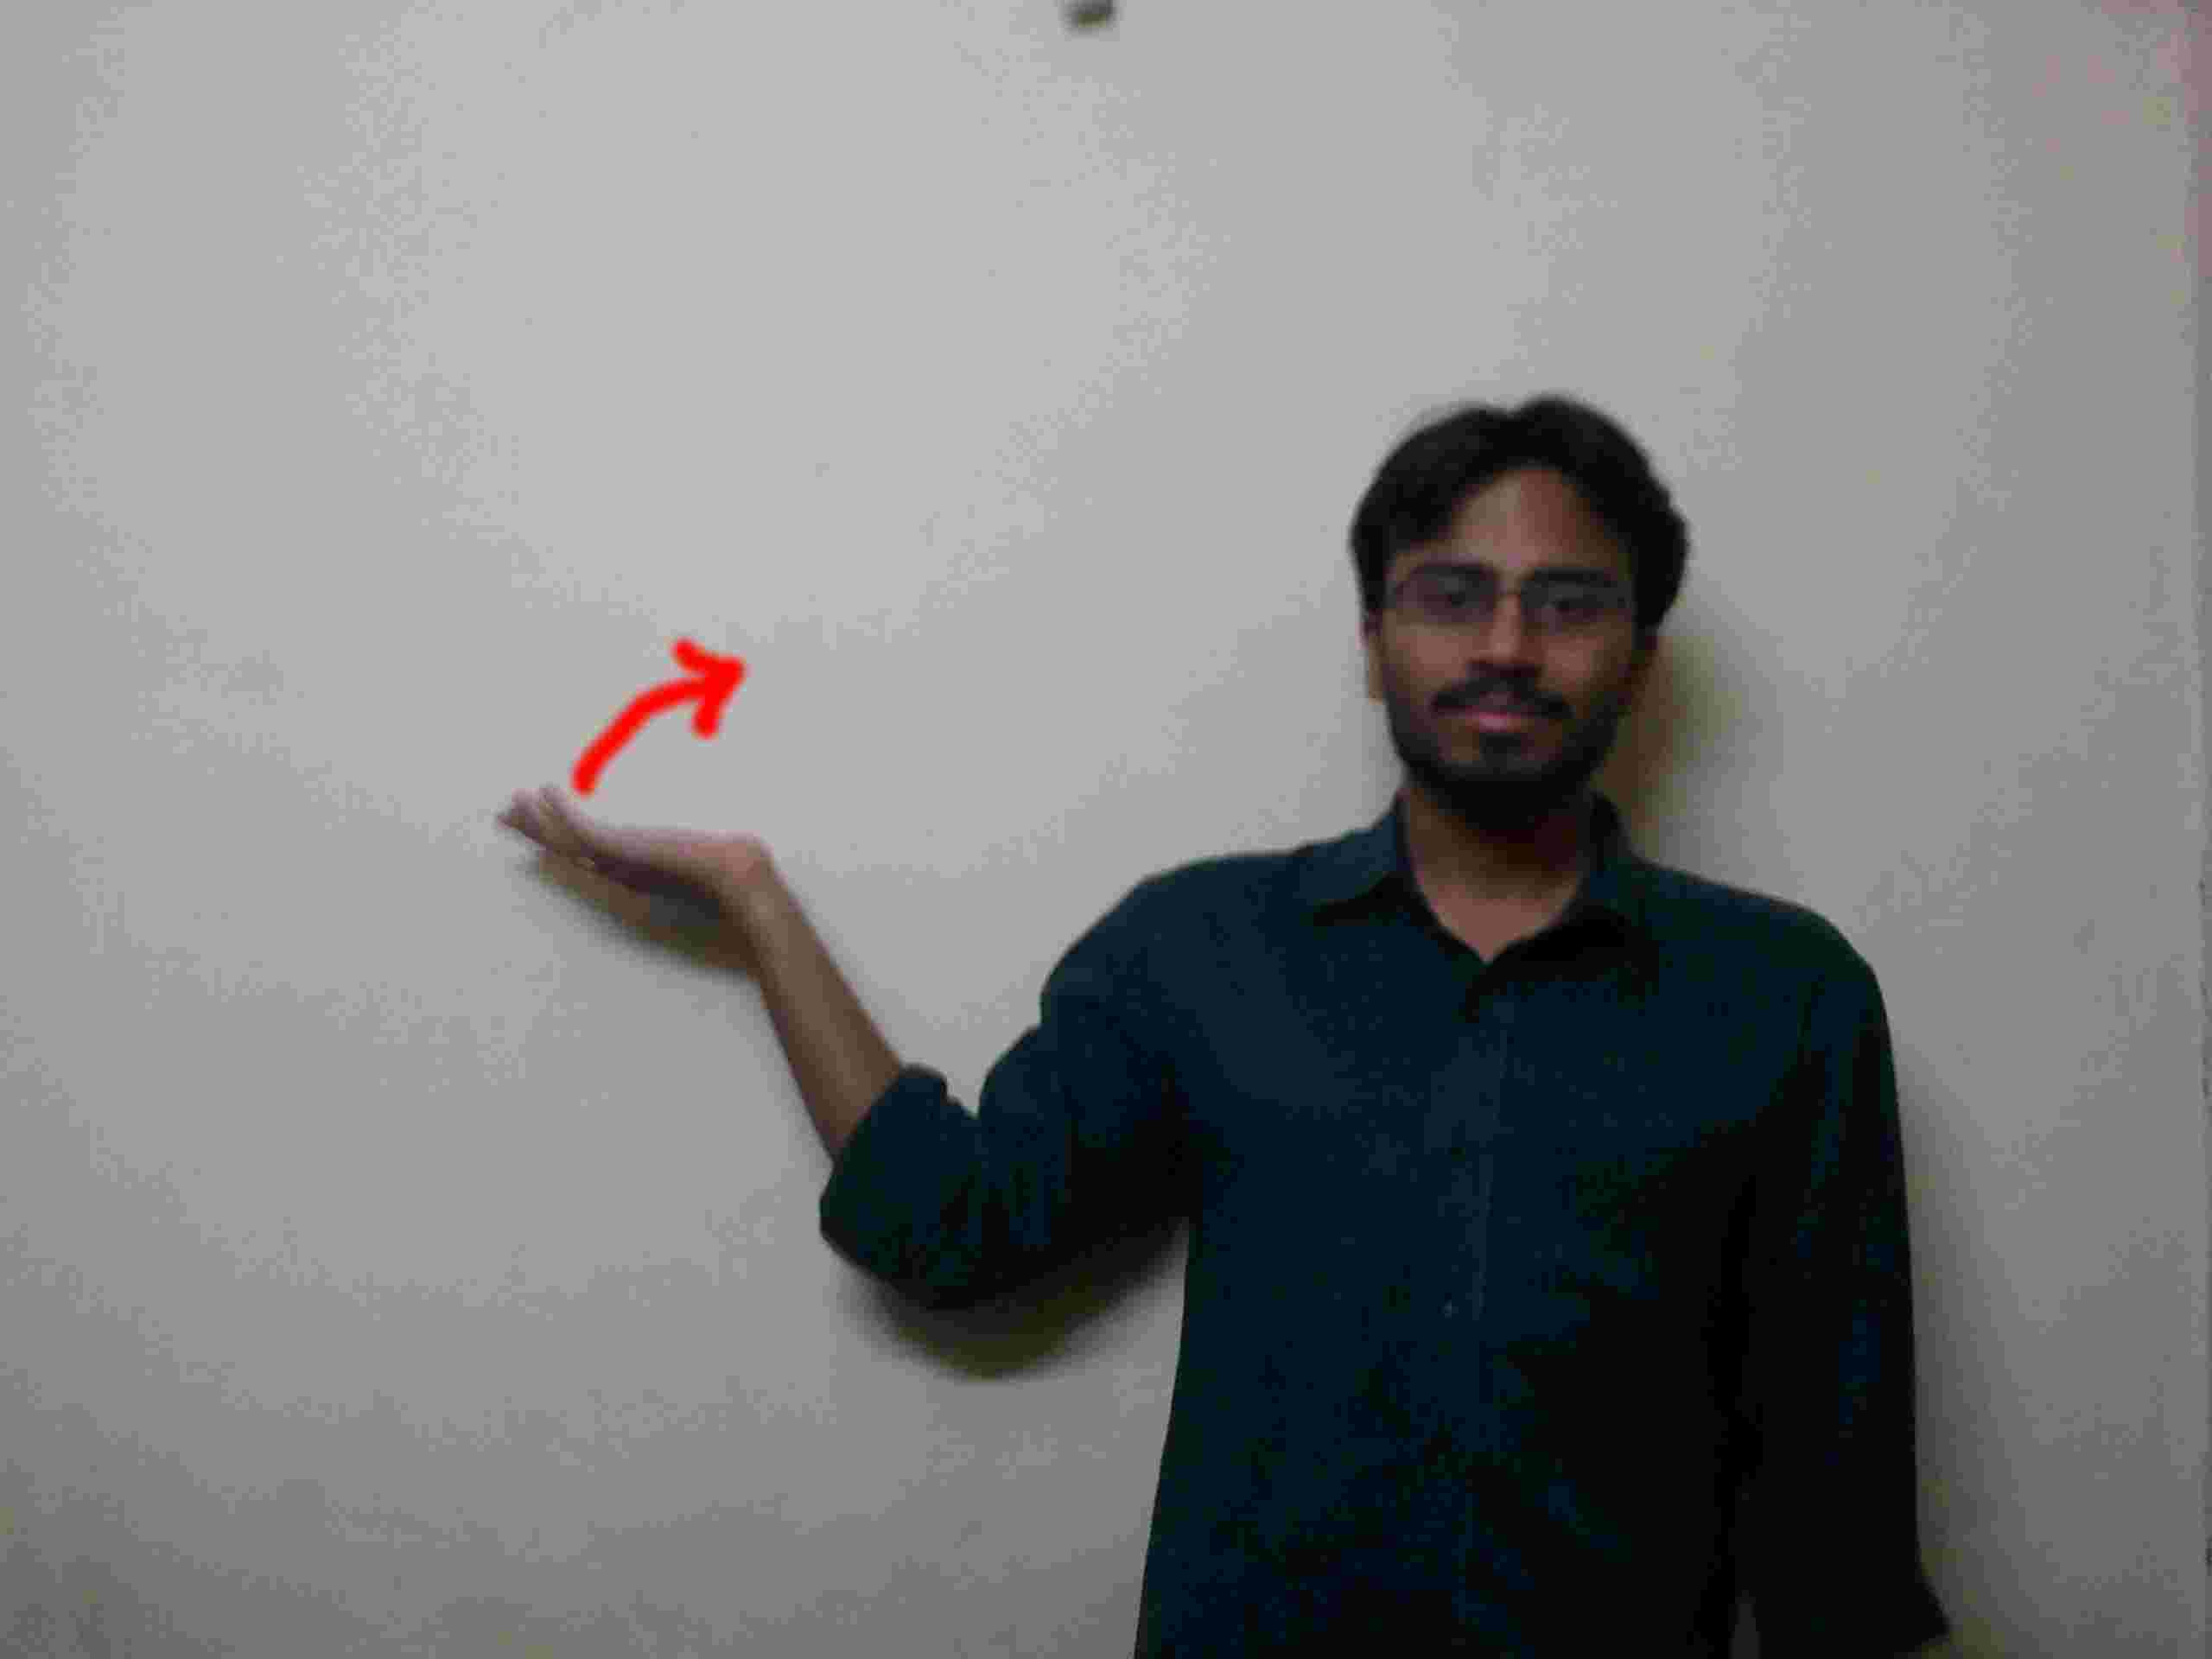
\includegraphics[scale = .06]{gestures/41.jpg} 
      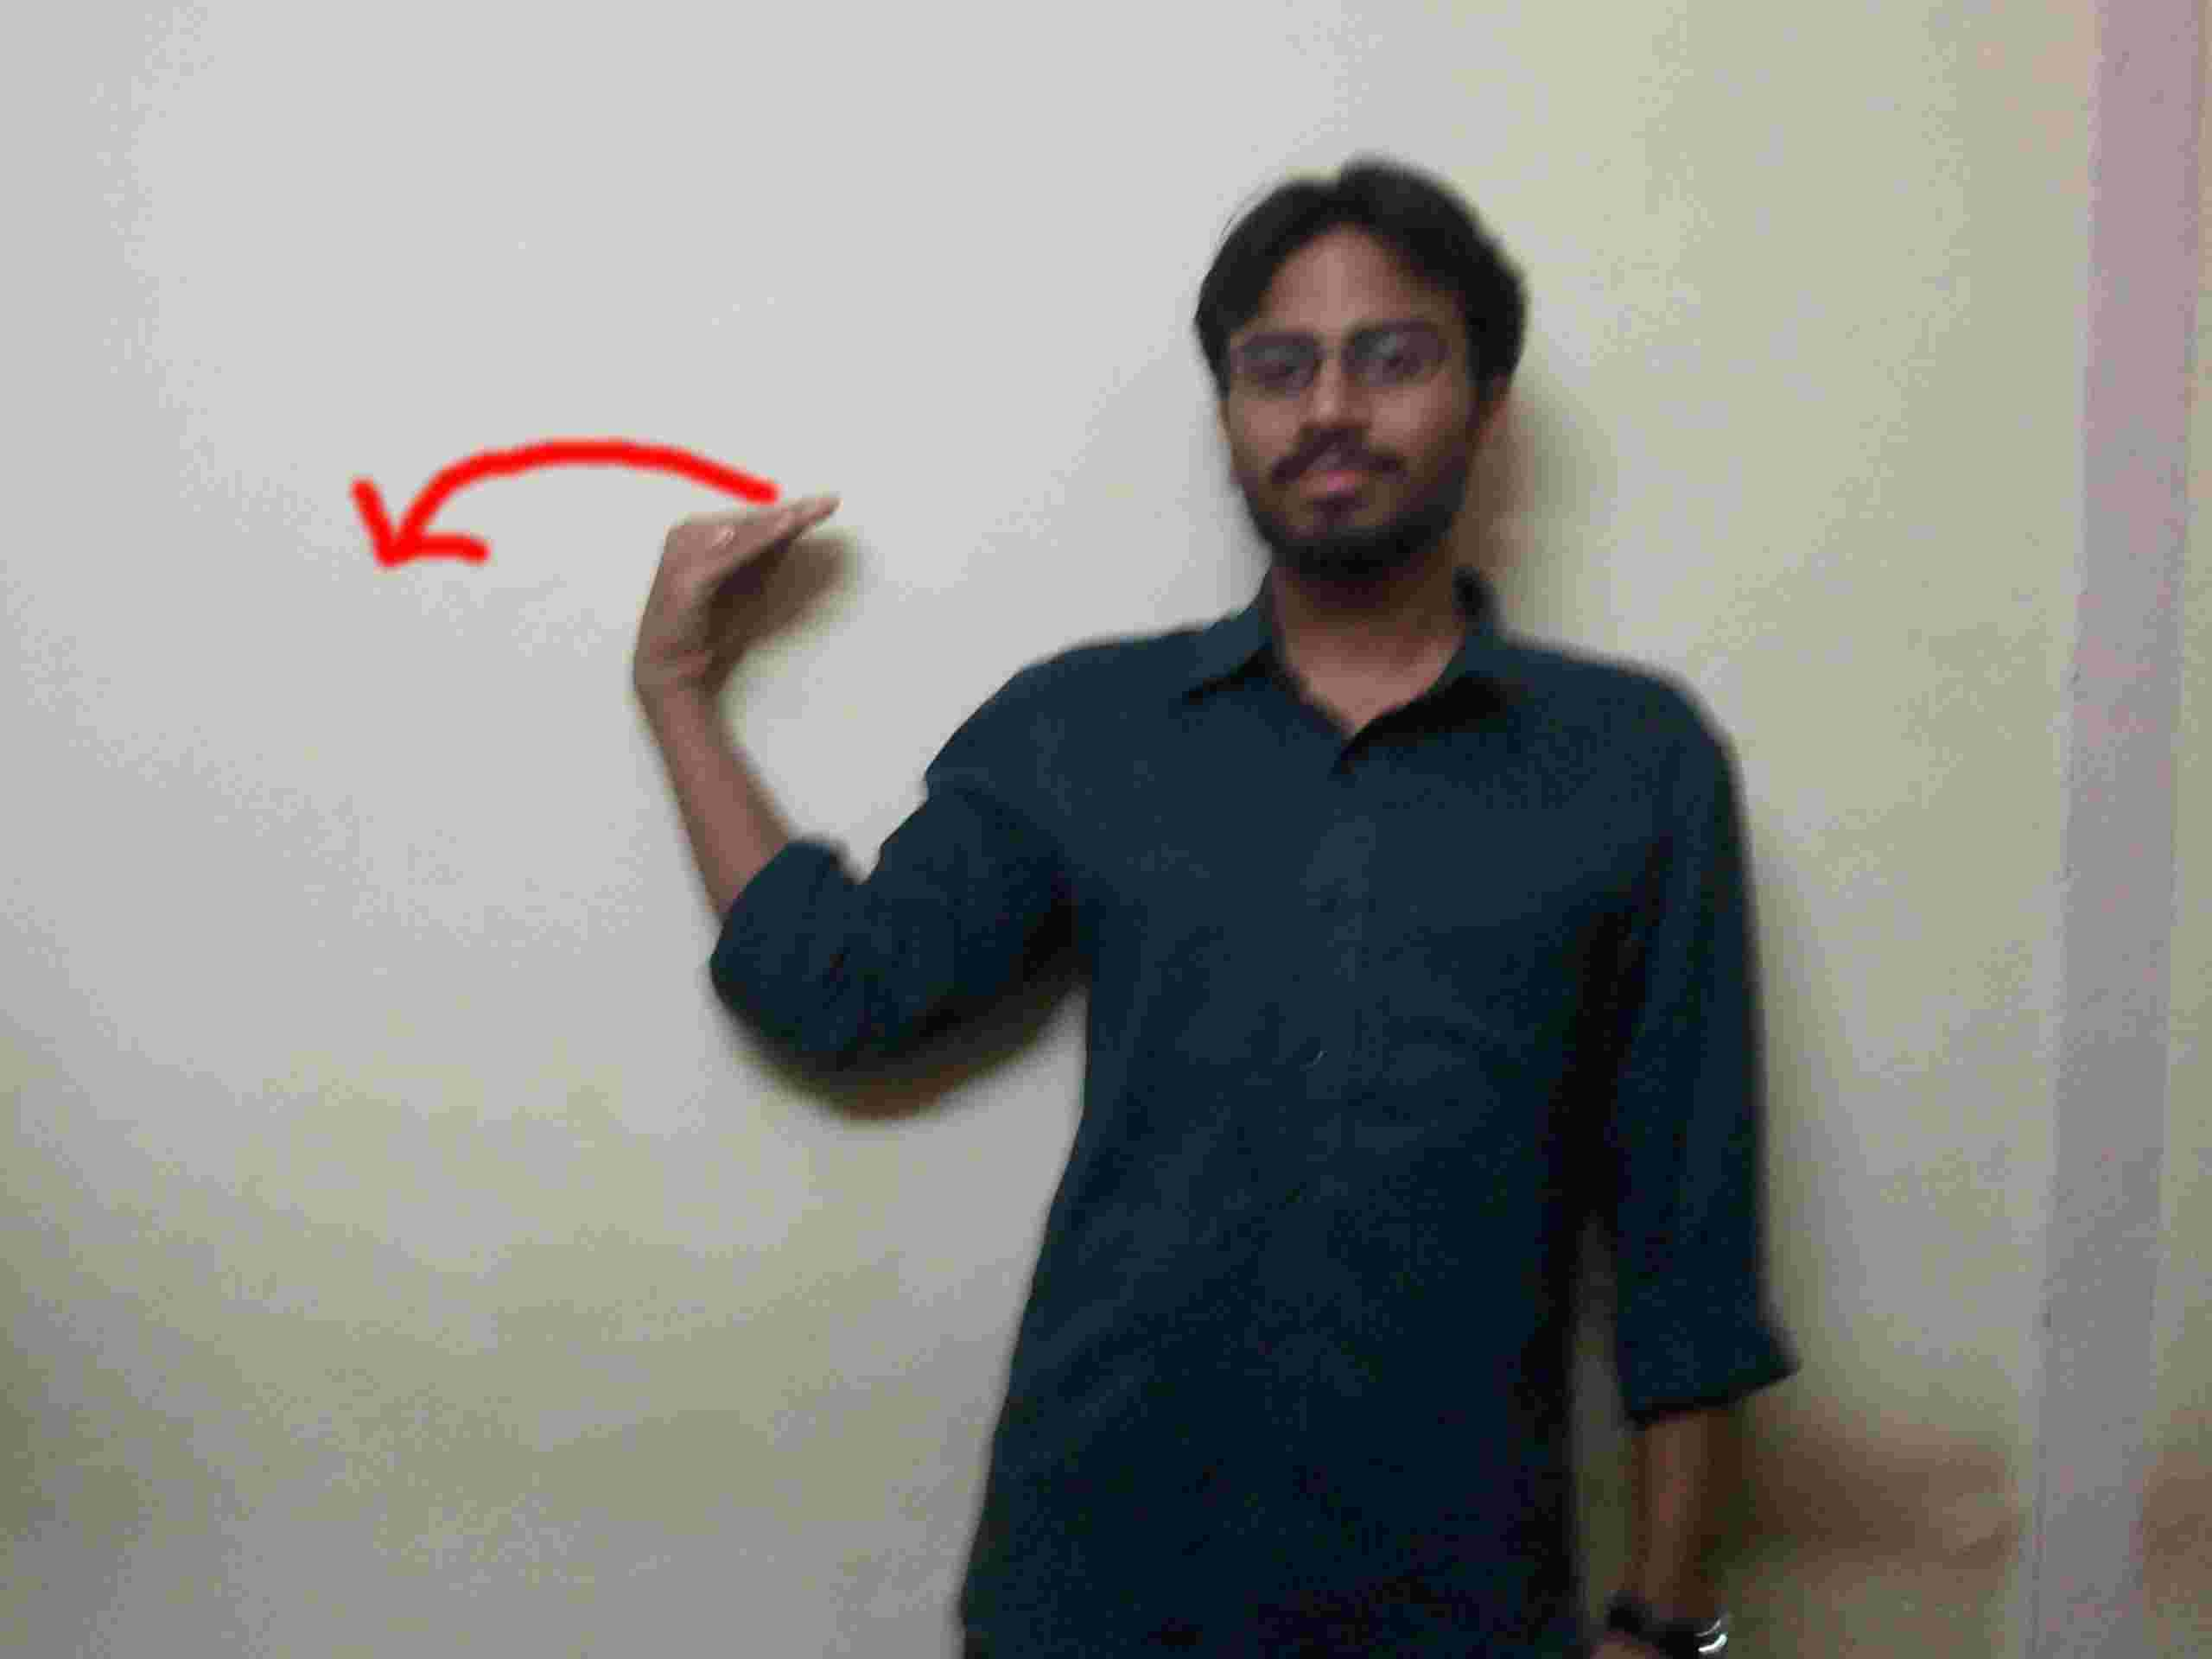
\includegraphics[scale = .06]{gestures/42.jpg} 
  \end{figure}
\end{frame}

\begin{frame}{5.Wrist Roll}
  \begin{figure}
      \centering
      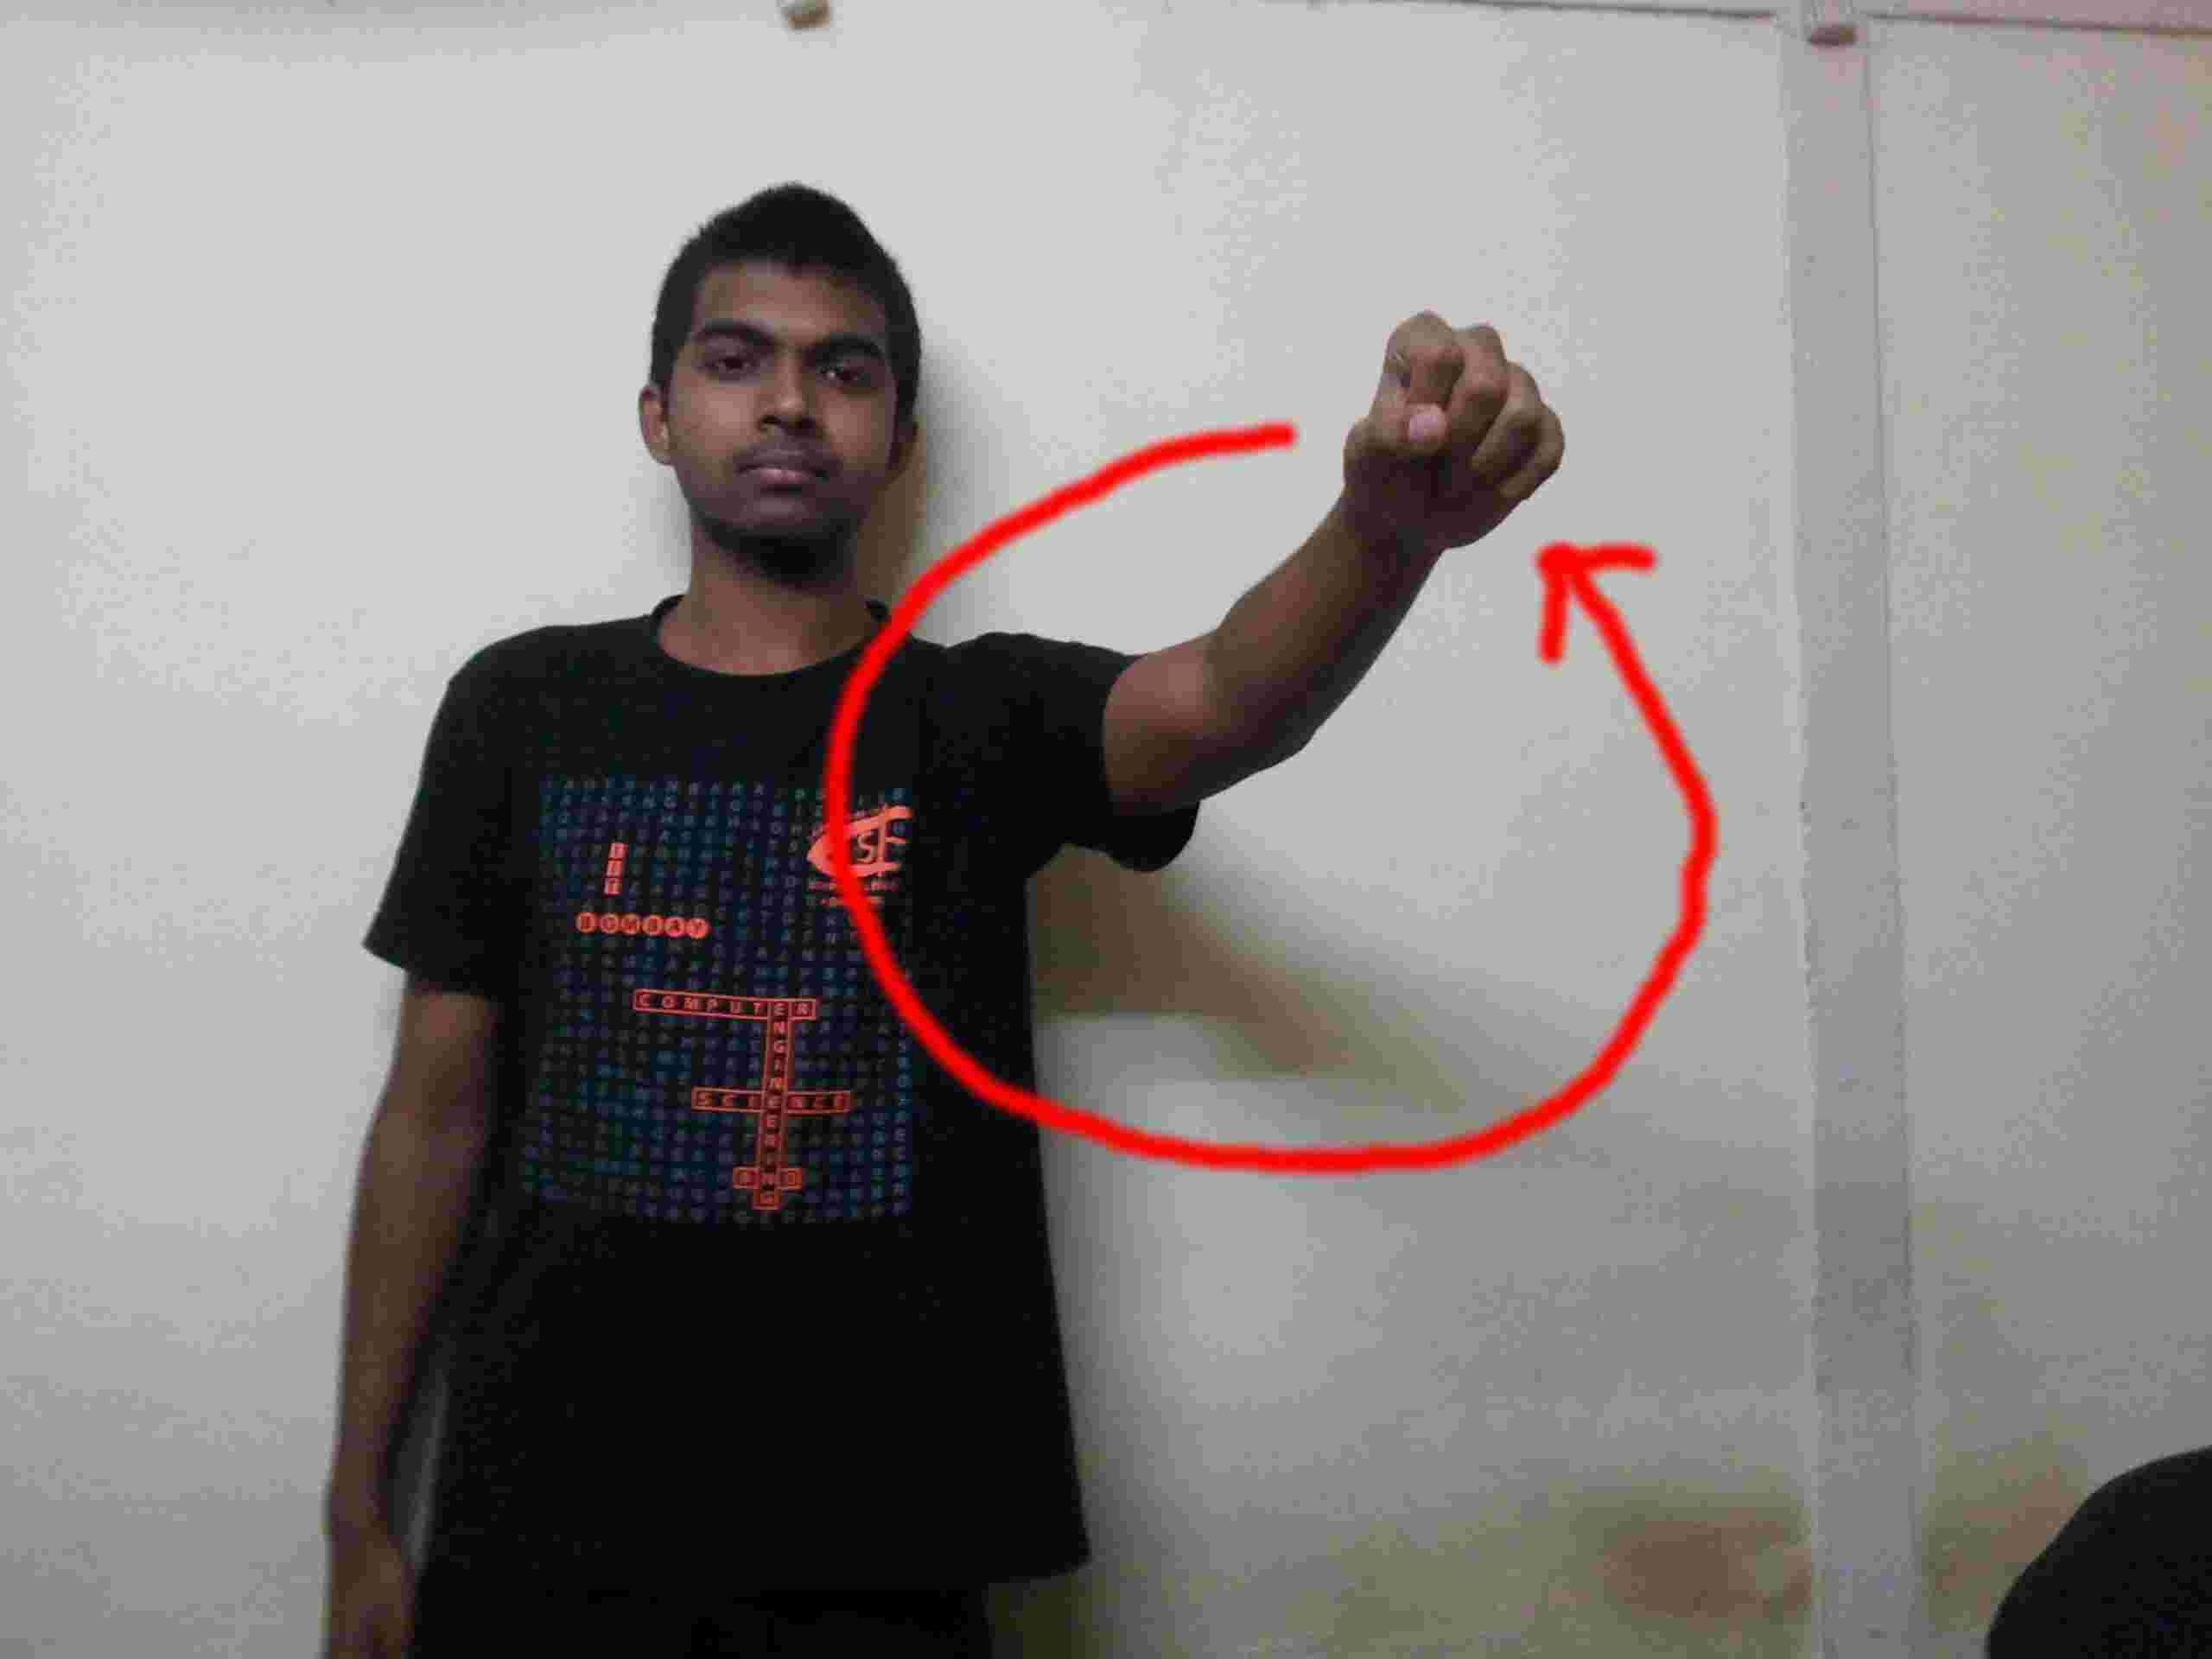
\includegraphics[scale = .08]{gestures/5.jpg} 
  \end{figure}
\end{frame}

\begin{frame}{6.Grip and Ungrip}
  \begin{figure}
      \centering
      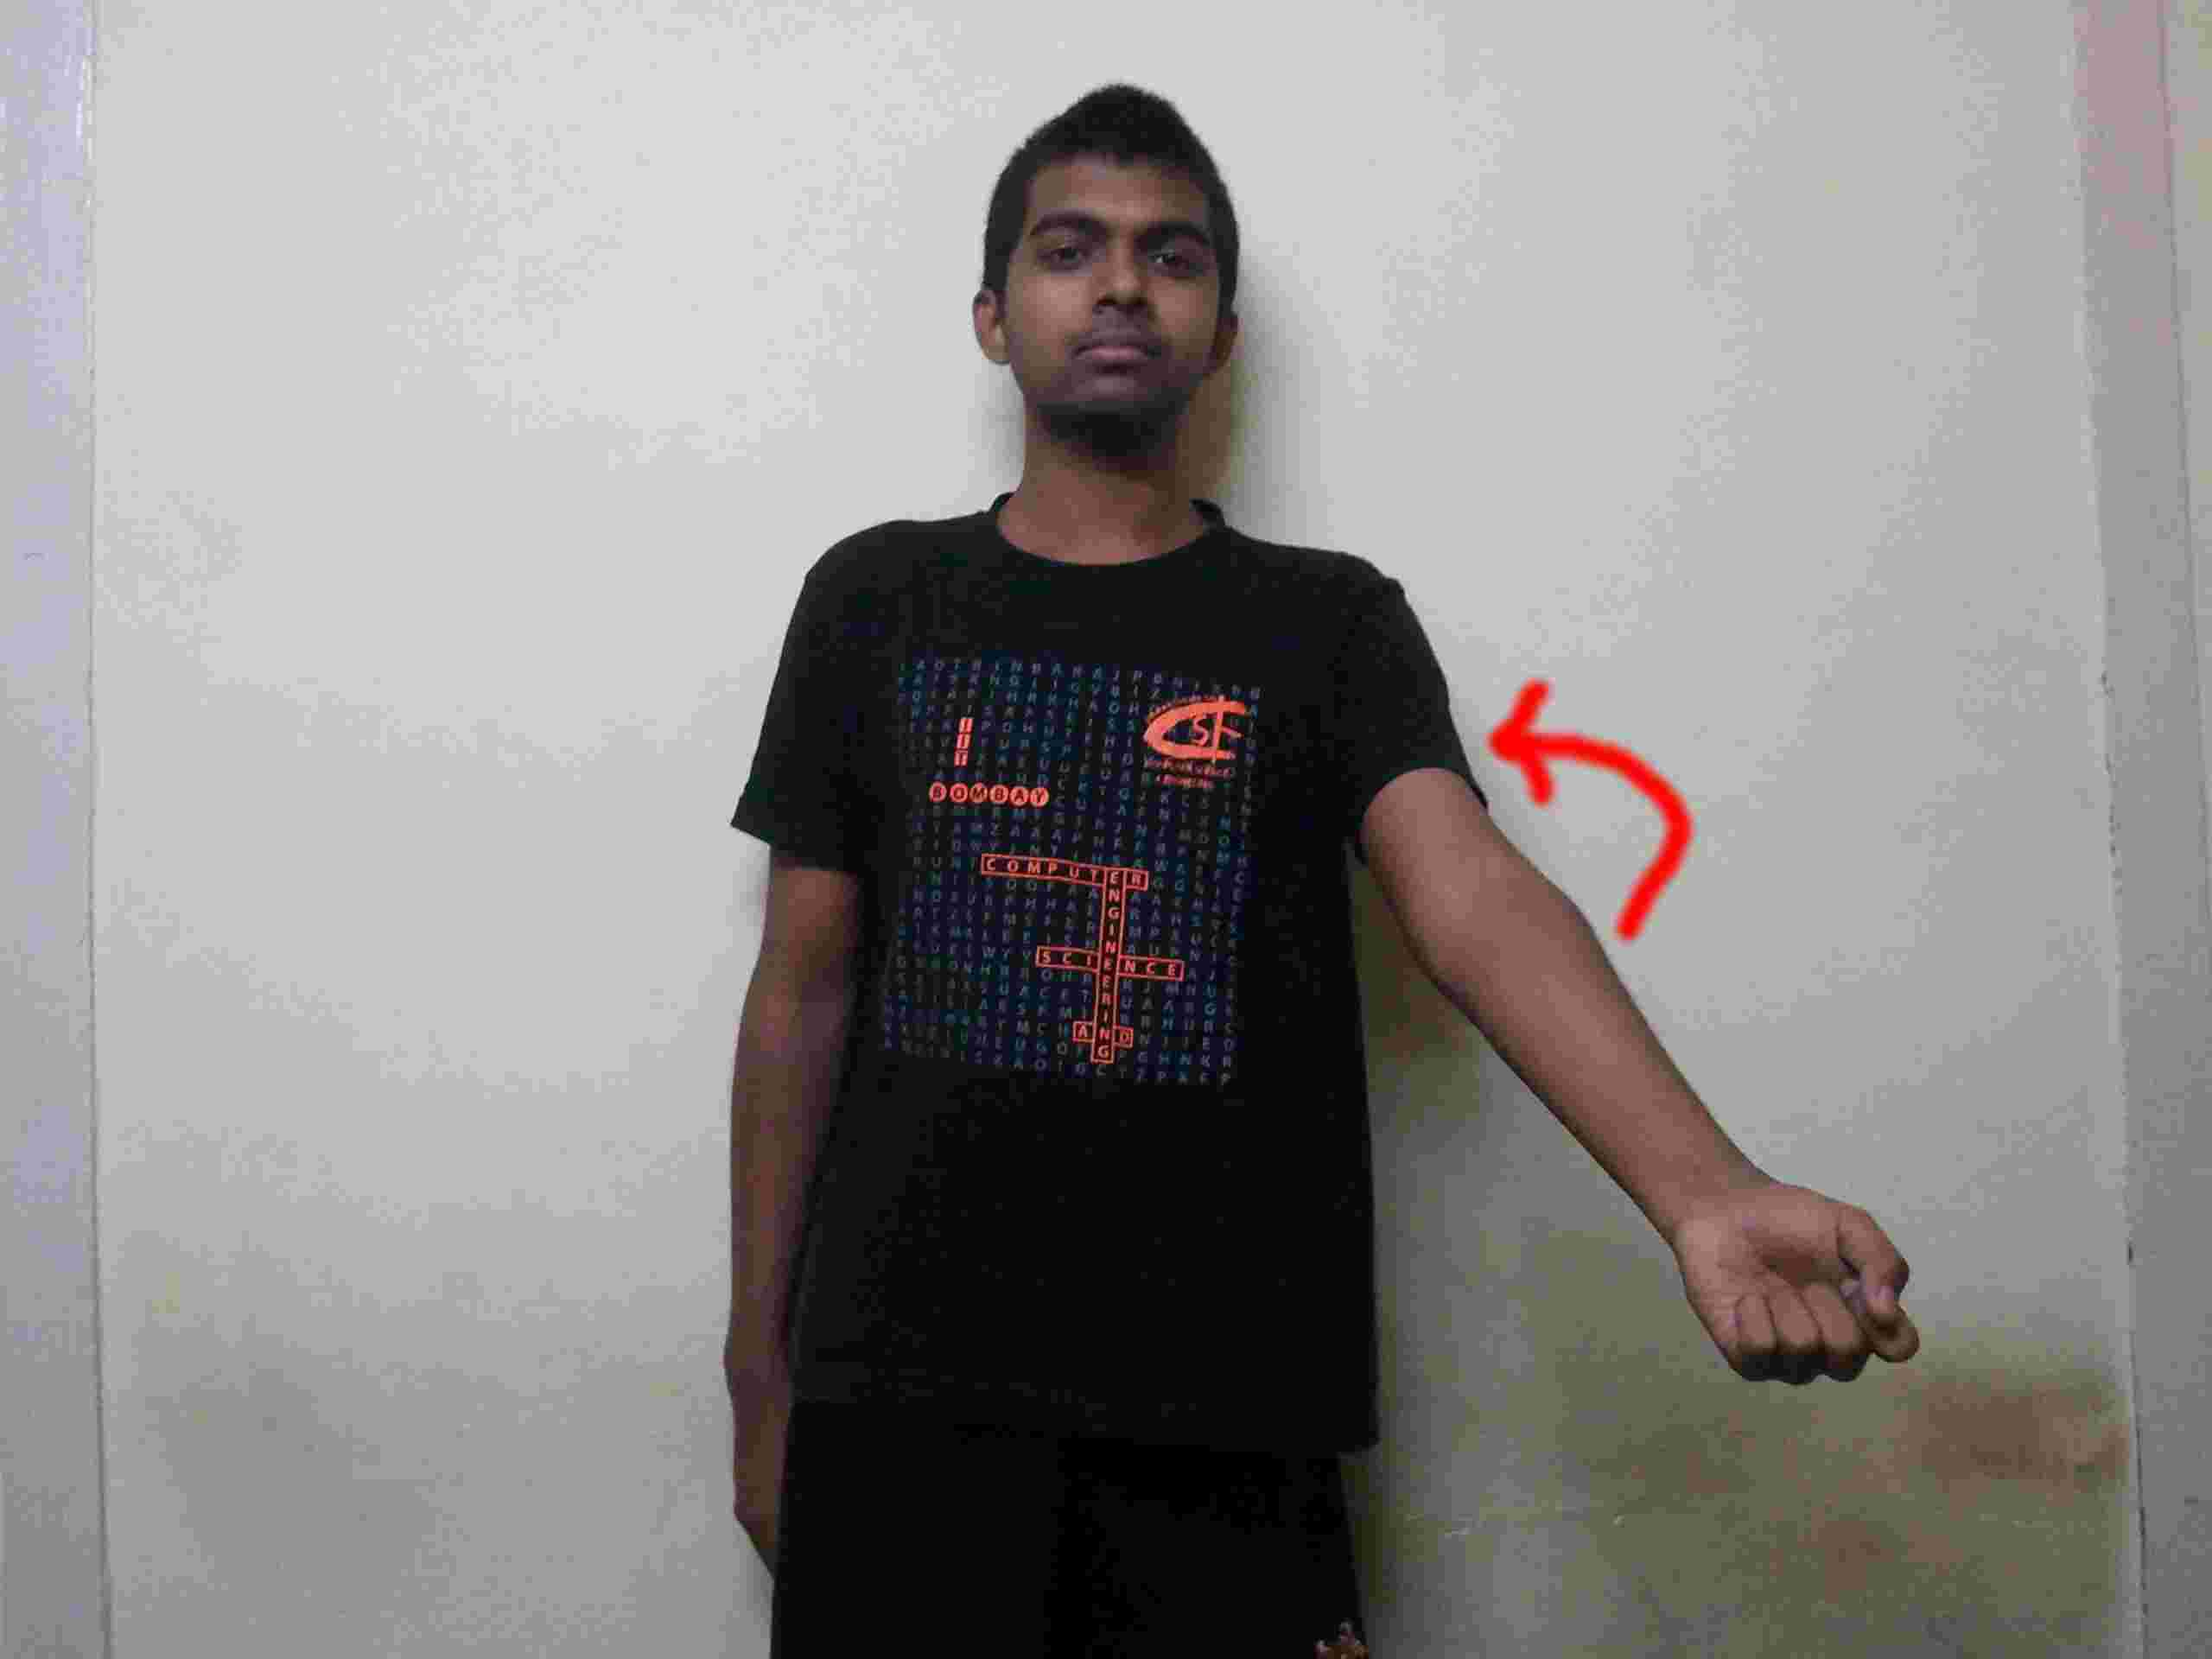
\includegraphics[scale = .06]{gestures/61.jpg} 
      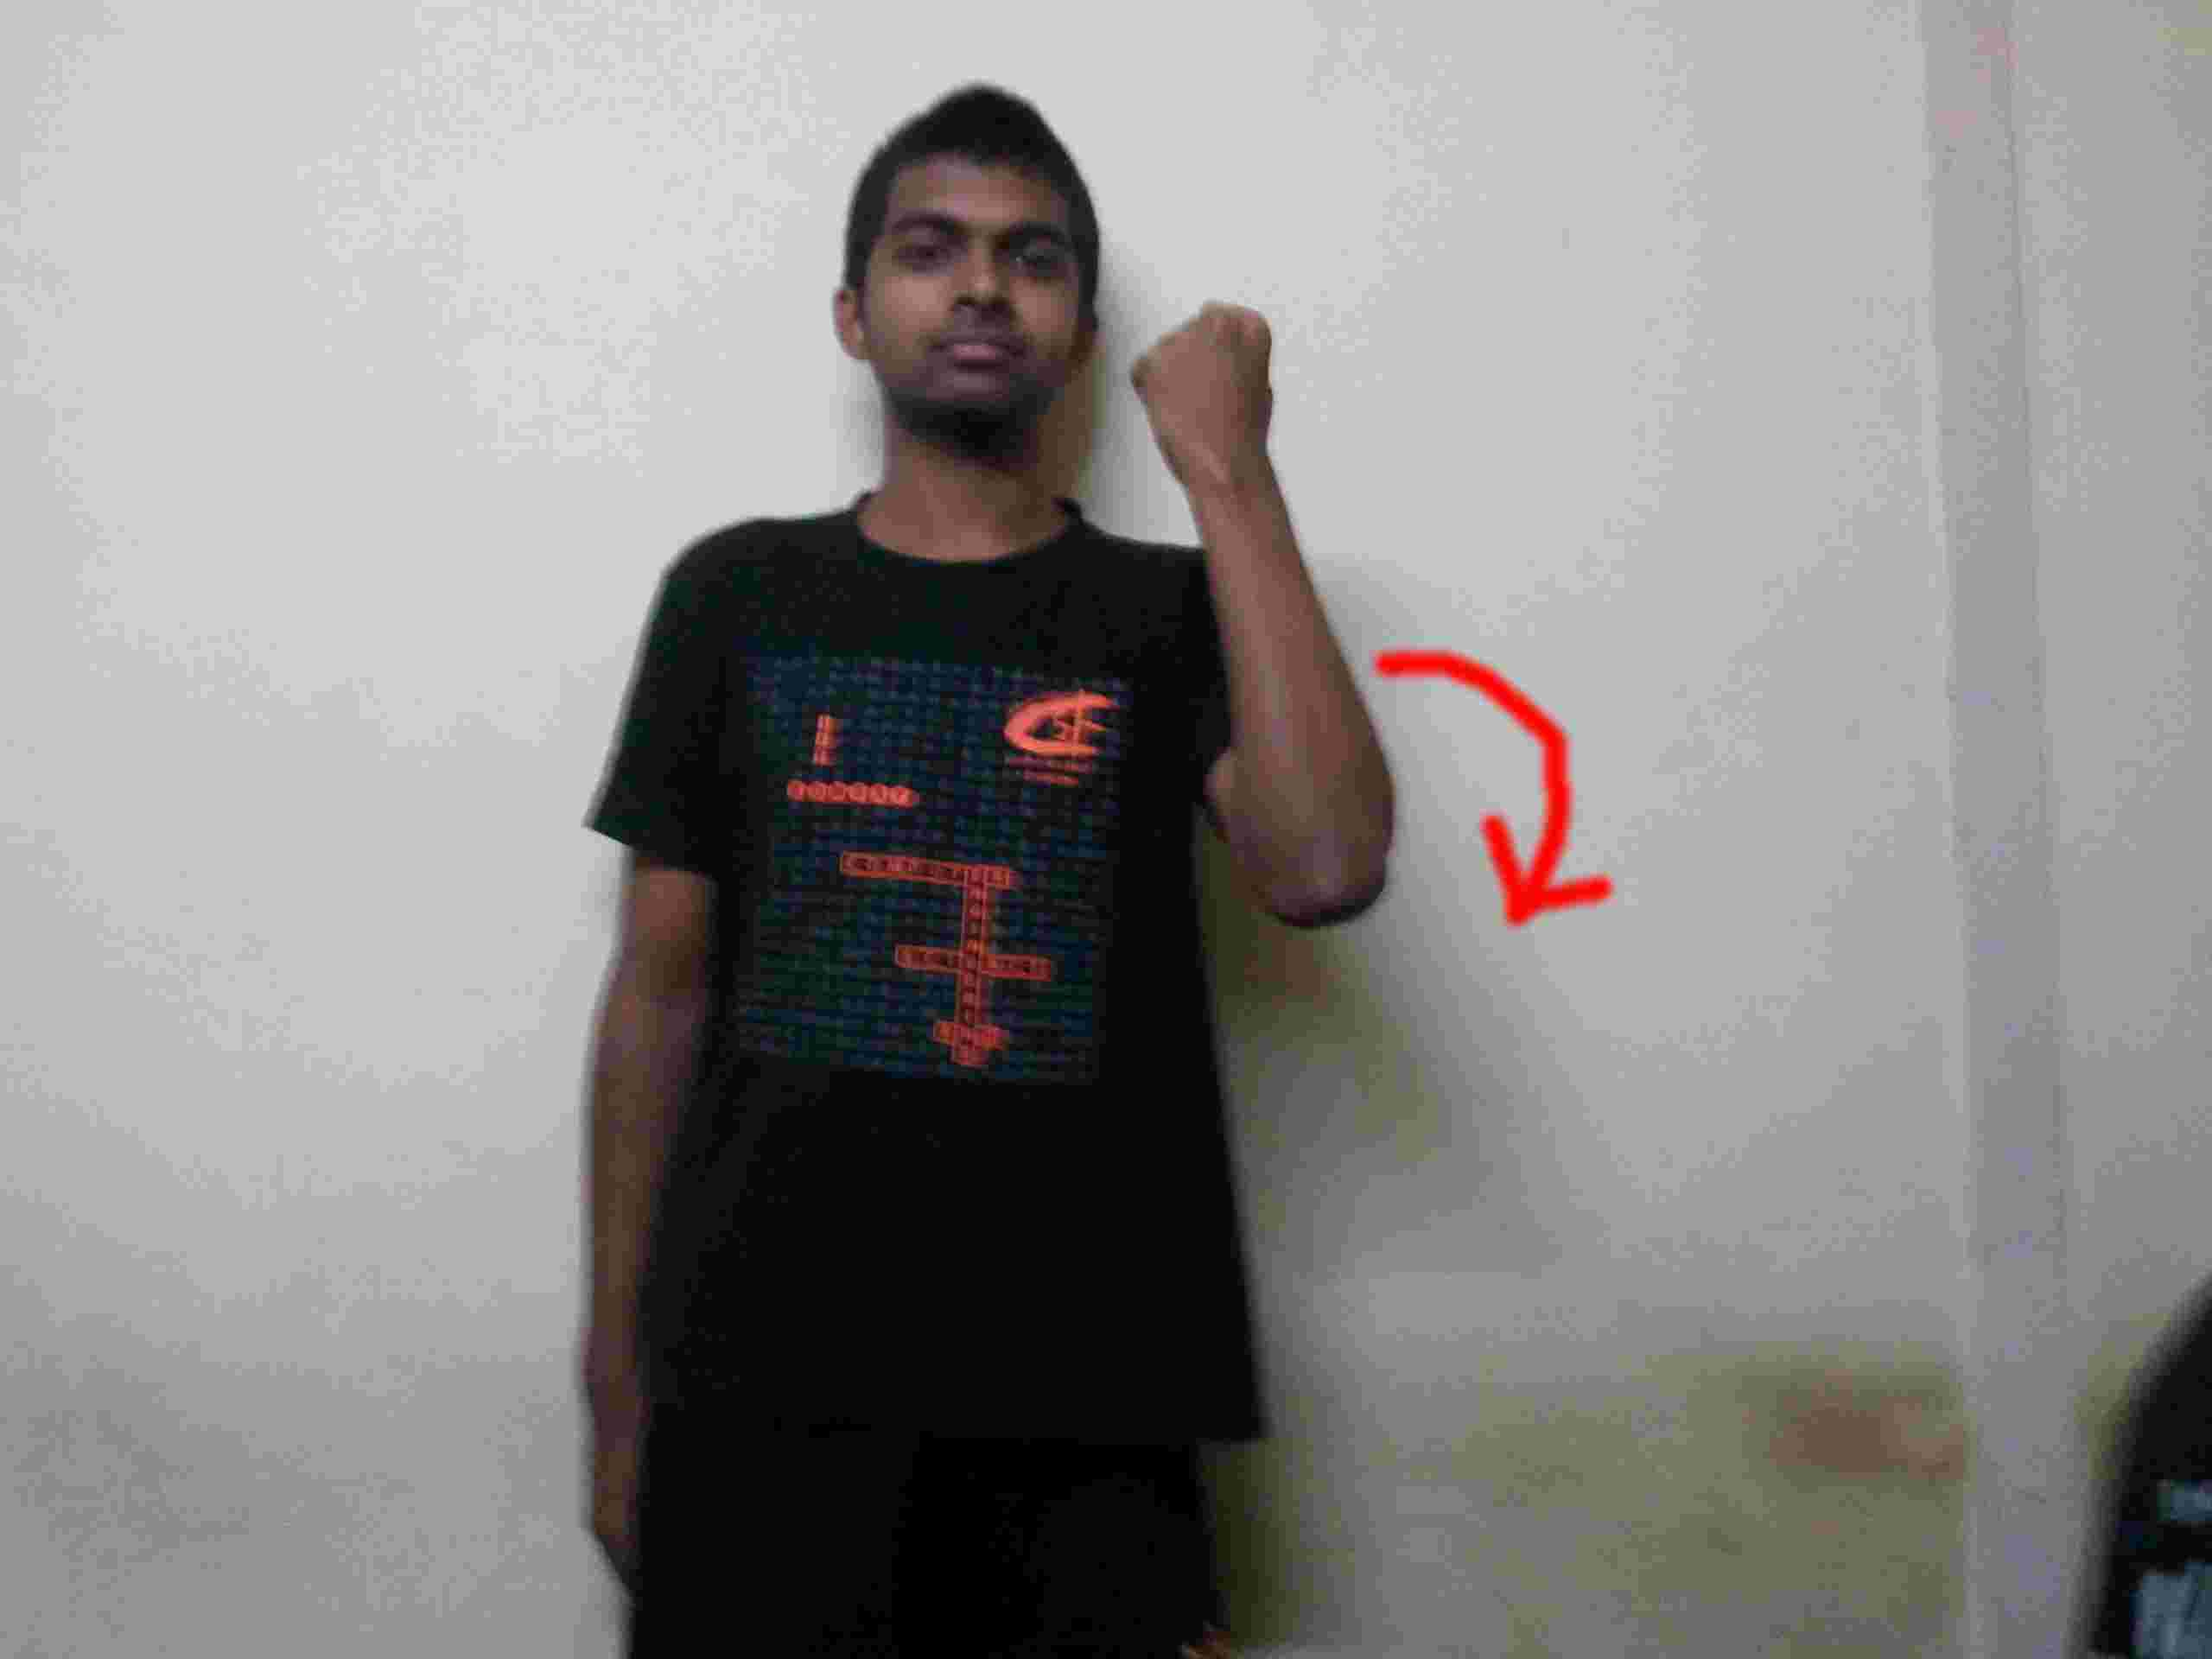
\includegraphics[scale = .06]{gestures/62.jpg} 
  \end{figure}
\end{frame}
\subsection{Wireless Control and Transmission}
\begin{frame}{Wireless Control and Transmission}
Attach a Zigbee module to the robotic arm
\begin{itemize}
\item[-] The livefeed from camera on the robotic arm is sent via Zigbee to the computer
\item[-] Instructions from the computer is sent to the robotic arm through the Zigbee module
\end{itemize}
\end{frame}

\section{Hardware}
\begin{frame}{Hardware Required}
\begin{itemize}
\item Kinect for Xbox v1
\item Dexter ER2 Robotic Arm
\item Camera
\item Zigbee Module
\end{itemize}
\end{frame}
\section{Risk}
\begin{frame}{Where can we fail}
\begin{itemize}
\item might be difficult to get live feed. Reasons:
\begin{itemize}
\item[-]Zigbee too slow to transmit good quality video
\item[-]Connecting camera and robotic arm may give trouble
\end{itemize}
\item Kinect may not accurately capture wrist movements.
\begin{itemize}
\item[-]use the other hand to control wrist movements
\end{itemize}
\end{itemize}
\end{frame}

\end{document}
